\documentclass[12pt]{article}

% ---------------------------------------------------------------------------
% Estimation and Inference on Two-Threshold Value Functionals
% ---------------------------------------------------------------------------
% Standalone-compilable companion to may_2026.tex ("Inference on Policy Value
% under Admissibility-Constrained Optimal Treatment Rules").  Designed to slot
% in as the "Estimation and Inference of the Value Functional" section of the
% JMP: it generalizes Chen, Chen & Gao (2025) [single threshold: plug-in,
% analytical variance, sieve-Riesz inference] and the extended draft
% [quadratic debiasing, sieve DML] to value functionals defined by TWO
% thresholds, and develops the combined (doubly debiased) procedure left open
% in Remark 7 of the extended draft.  Macros match may_2026.tex.
% ---------------------------------------------------------------------------

\usepackage[margin=1in]{geometry}
\usepackage{setspace}
\usepackage{amsmath,amssymb,amsthm,mathtools,bm}
\usepackage{enumitem}
\usepackage{natbib}
\usepackage[colorlinks=true,linkcolor=blue,citecolor=blue,urlcolor=blue]{hyperref}
\usepackage{booktabs}
\usepackage{longtable}
\usepackage{graphicx}
\usepackage{microtype}
\usepackage{bbm}

\onehalfspacing

\newtheorem{theorem}{Theorem}[section]
\newtheorem{proposition}[theorem]{Proposition}
\newtheorem{lemma}[theorem]{Lemma}
\newtheorem{corollary}[theorem]{Corollary}
\newtheorem{assumption}[theorem]{Assumption}
\newtheorem{definition}[theorem]{Definition}
\newtheorem{remark}[theorem]{Remark}
\newtheorem{example}[theorem]{Example}

\newcommand{\R}{\mathbb{R}}
\newcommand{\E}{\mathbb{E}}
\newcommand{\Prob}{\mathbb{P}}
\newcommand{\1}{\mathbbm{1}}
\newcommand{\dd}{\,\mathrm{d}}
\newcommand{\Haus}{\mathcal{H}}
\newcommand{\norm}[1]{\left\lVert #1 \right\rVert}
\newcommand{\abs}[1]{\left\lvert #1 \right\rvert}
\newcommand{\inner}[2]{\left\langle #1, #2 \right\rangle}
\newcommand{\argmax}{\operatorname*{arg\,max}}
\newcommand{\Th}{\Theta}
\newcommand{\Mg}{\mathcal{M}_{g}}
\newcommand{\Mh}{\mathcal{M}_{h}}
\newcommand{\Corner}{\mathcal{C}}

\title{Estimation and Inference on Two-Threshold Value Functionals\thanks{%
This section extends the single-threshold framework of Chen, Chen, and Gao
(2025) and its debiased-estimation companion to value functionals defined by
the intersection of two estimated decision boundaries. It is written to be
self-contained; notation follows the JMP draft \texttt{may\_2026.tex}.}}
\author{Zhenxiao Chen\thanks{Department of Economics, University of
Pennsylvania, USA, zxchen@upenn.edu.}}
\date{\today}

\begin{document}
\maketitle

\begin{abstract}
\noindent We study estimation and inference for value functionals of the form
$\Th_{0}=\E\big[\1\{g_{0}(X)\geq0\}\,\1\{h_{0}(X)\geq0\}\,v_{0}(X)\big]$,
where $g_{0}$ and $h_{0}$ are two nonparametric contrast functions estimated
from the same experiment. Such \emph{two-threshold} functionals arise whenever
a planner imposes a pointwise admissibility screen on top of a benefit margin:
leading examples are the share of the population that benefits in the short
run but is harmed in the long run under a surrogate-index treatment rule
(Athey, Chetty, Imbens, and Kang, 2024), and treatment-path welfare components
of an optimal dynamic regime. We generalize the single-threshold theory of
Chen, Chen, and Gao (2025): the pathwise derivative is a sum of \emph{two}
boundary (Hausdorff) integrals, the plug-in estimator converges at the
one-dimensional nonparametric rate $n^{-s/(2s+1)}$ (attained under
$s\geq d$), and a two-band sieve-Riesz
variance estimator delivers valid studentized inference. Our main new result
characterizes the \emph{second-order} pathwise derivative: in addition to two
margin curvature terms it contains a codimension-two \emph{corner} integral
over $\{g_{0}=0\}\cap\{h_{0}=0\}$ whose ``diagonal'' contribution to the
plug-in expansion is of the same order $K_{n}/n$ as the margin diagonals.
Consequently, margin-by-margin quadratic debiasing \`{a} la Chen and Gao
(2026) is insufficient in the two-threshold setting; we construct
corner-aware split-sample and leave-one-out debiased estimators that attain
the minimax rate under the weaker smoothness $s>(d+1)/2$, and give a
tuning-free half-sample jackknife representation of the split-sample
correction. Finally, we combine the quadratic correction with a cross-fitted
sieve-Riesz first-order correction into a \emph{doubly debiased} estimator
that simultaneously accommodates generic machine-learning first stages and
weak smoothness --- the combination posed as an open question in the
single-threshold setting. Monte Carlo experiments calibrated to the
Banerjee et al.\ (2015) graduation experiment, following the Wasserstein-GAN
calibration protocol of Chen and Ritzwoller (2023), corroborate the theory
and delineate its finite-sample limits for machine-learning first stages.
\end{abstract}

\section{Setup and Examples}\label{sec:setup}

\subsection{Data and estimands}

The observed data are an i.i.d.\ sample
$\{Z_{i}=(X_{i},W_{i},S_{i},Y_{i})\}_{i=1}^{n}$, where $X_{i}\in\mathcal
X\subset\R^{d}$ are covariates with density $f_{0}$ on a bounded rectangular
support, $W_{i}\in\{0,1\}$ is a binary treatment with
$(S_{i}(0),S_{i}(1),Y_{i}(0),Y_{i}(1))\perp W_{i}\mid X_{i}$ and overlap
$p_{0}(x):=\E[W_{i}\mid X_{i}=x]\in(0,1)$, $S_{i}$ is a short-run outcome
(or surrogate), and $Y_{i}$ is a long-run outcome. Define the arm means and
contrasts
\begin{align}
\mu_{S,0}(x,w):=\E[S_{i}\mid X_{i}=x,W_{i}=w], \qquad
\tau_{S}(x):=\mu_{S,0}(x,1)-\mu_{S,0}(x,0), \label{eq:tauS}\\
\mu_{Y,0}(x,w):=\E[Y_{i}\mid X_{i}=x,W_{i}=w], \qquad
\tau_{Y}(x):=\mu_{Y,0}(x,1)-\mu_{Y,0}(x,0). \label{eq:tauY}
\end{align}
Throughout we write $\gamma_{0}:=(g_{0},h_{0})$ for a generic pair of
identified contrast functions built from
$(\mu_{S,0},\mu_{Y,0})$ --- in the leading example $g_{0}=\tau_{S}$ and
$h_{0}=-\tau_{Y}$ --- and consider the \emph{two-threshold value functional}
\begin{equation}
\Th(\gamma_{0})
:=\int_{\mathcal X}\1\{g_{0}(x)\geq0\}\,\1\{h_{0}(x)\geq0\}\,
v_{0}(x)\,f(x)\dd x,
\label{eq:Theta}
\end{equation}
where $v_{0}$ is a known, user-chosen value weight and $f$ is the covariate
density of the target population. As in the single-threshold analysis we
distinguish the \emph{known-density} case ($f$ given, integral computed
numerically) and the \emph{empirical} case ($f=f_{0}$ unknown, integral
replaced by the sample average $n^{-1}\sum_{i}\1\{\cdot\}v_{0}(X_{i})$); the
asymptotic theory is identical in both because the additional sampling error
of the empirical measure is $O_{p}(n^{-1/2})$, which is negligible relative
to the slower boundary-driven rate of \eqref{eq:Theta}.

\subsection{Leading examples}

\begin{example}[Surrogate-induced harm share]\label{ex:harm}
A planner who observes only the short-run outcome adopts the surrogate-index
rule ``treat iff $\tau_{S}(x)\geq0$.'' The long-run criterion would instead
require $\tau_{Y}(x)\geq0$. With $g_{0}=\tau_{S}$, $h_{0}=-\tau_{Y}$, and
$v_{0}\equiv1$, \eqref{eq:Theta} becomes
\[
\theta_{0}=\Prob_{f}\big(\tau_{S}(X)\geq 0,\ \tau_{Y}(X)\leq 0\big),
\]
the mass of the population that the surrogate rule treats but that is harmed
in the long run --- a direct diagnostic of the surrogate-index approach of
Athey, Chetty, Imbens, and Kang (2024). This is the functional we take to the
calibrated Monte Carlo of Section~\ref{sec:mc}.
\end{example}

\begin{example}[Admissibility-constrained policy value]\label{ex:admiss}
In the two-item-checklist planner problem of the JMP draft, a hard
admissibility screen $g_{0}(x)\geq0$ (e.g.\ no expected severe side effect)
is imposed before the benefit margin $h_{0}(x)\geq0$; treated-population
aggregates take the form \eqref{eq:Theta} with $v_{0}$ equal to a utility,
cost, or eligibility weight.
\end{example}

\begin{example}[Dynamic treatment-path welfare]\label{ex:dtr}
The $(1,1)$ path-welfare component of an optimal two-stage dynamic regime,
$V_{11}^{*}=\E[Y^{(1,1)}\1\{\kappa(S)\geq0\}\1\{\delta(X^{(1)})\geq0\}]$,
has the same two-threshold structure, with the additional complication that
the first-stage contrast $\kappa$ is itself a functional of the second-stage
threshold. The static analysis of this section is the template for that case;
the extra ``moving-boundary-within-a-moving-boundary'' terms are treated in
the DTR section of the draft.
\end{example}

\subsection{Geometry and maintained assumptions}

Write $w(x):=v_{0}(x)f(x)$ for the boundary weight, and define the two
\emph{margins} and the \emph{corner}
\begin{equation}
\Mg:=\{x:g_{0}(x)=0,\ h_{0}(x)>0\},\qquad
\Mh:=\{x:h_{0}(x)=0,\ g_{0}(x)>0\},\qquad
\Corner:=\{x:g_{0}(x)=h_{0}(x)=0\}.
\label{eq:margins}
\end{equation}

\begin{assumption}[Model]\label{ass:model}
(a) $\{Z_{i}\}$ is i.i.d.; $\mathcal X$ is bounded rectangular; overlap holds;
(b) $\mu_{S,0}(\cdot,w),\mu_{Y,0}(\cdot,w)\in\Lambda^{s}(\mathcal X)$ (H\"older
class) with $s>1$, for $w\in\{0,1\}$; (c) the conditional second moments
$\sigma_{S}^{2}(x,w),\sigma_{Y}^{2}(x,w)$ of the regression residuals
$\epsilon_{S,i}:=S_{i}-\mu_{S,0}(X_{i},W_{i})$,
$\epsilon_{Y,i}:=Y_{i}-\mu_{Y,0}(X_{i},W_{i})$ are bounded and bounded away
from zero, and the conditional correlation
$\rho_{SY}(x,w):=\mathrm{Corr}(\epsilon_{S,i},\epsilon_{Y,i}\mid
X_{i}=x,W_{i}=w)$ is well defined; (d) $v_{0}$ is bounded and continuously
differentiable, and $f$ is bounded with bounded gradient, absolutely
continuous w.r.t.\ $f_{0}$ with bounded Radon--Nikodym derivative.
\end{assumption}

\begin{assumption}[Regular margins and transversal corner]\label{ass:geometry}
$g_{0}$ and $h_{0}$ are twice continuously differentiable in neighborhoods of
$\{g_{0}=0\}$ and $\{h_{0}=0\}$ respectively, with
(a) $\norm{\nabla g_{0}(x)}\geq\underline c>0$ on $\{g_{0}=0\}$ and
$\norm{\nabla h_{0}(x)}\geq\underline c>0$ on $\{h_{0}=0\}$;
(b) (\emph{transversality}) on $\Corner$, the angle $\omega(x)$ between
$\nabla g_{0}(x)$ and $\nabla h_{0}(x)$, defined by $\cos\omega(x)
=\inner{\nabla g_{0}}{\nabla h_{0}}/(\norm{\nabla g_{0}}\norm{\nabla h_{0}})$,
satisfies $\abs{\sin\omega(x)}\geq\underline c_{T}>0$;
(c) $\Haus^{d-1}(\Mg)+\Haus^{d-1}(\Mh)<\infty$ and
$\Haus^{d-2}(\Corner)<\infty$;
(d) the level sets $\{g_{0}=0\}$ and $\{h_{0}=0\}$ are contained in the
interior of the support of $w$ (equivalently, $w$ vanishes in a
neighborhood of $\partial\mathcal X$), so that no margin meets the edge of
the covariate support and the boundary calculus below involves only the
margins and their common corner.
\end{assumption}

Under Assumption~\ref{ass:geometry}, $\Mg$ and $\Mh$ are
$(d-1)$-dimensional $C^{2}$ submanifolds-with-boundary whose common relative
boundary is the $(d-2)$-dimensional corner $\Corner$ (a finite set of points
when $d=2$; empty when $d=1$ or when the constraints never bind jointly).
Transversality rules out tangential intersections, at which the corner would
inflate to a higher-dimensional set and the second-order calculus below would
fail.

\section{First-Order Theory}\label{sec:first}

\subsection{Pathwise derivative: two boundary integrals}

For directions $(u,v)$ (perturbations of $(g_{0},h_{0})$ induced by
perturbations of the four arm means), let
$\gamma_{t}:=(g_{0}+tu,\;h_{0}+tv)$.

\begin{proposition}[First derivative]\label{prop:D1}
Under Assumptions~\ref{ass:model}--\ref{ass:geometry},
\begin{equation}
D\Th(\gamma_{0})[u,v]
:=\frac{\dd}{\dd t}\Th(\gamma_{t})\Big|_{t=0}
=\int_{\Mg}\frac{u(x)\,w(x)}{\norm{\nabla g_{0}(x)}}\dd\Haus^{d-1}(x)
+\int_{\Mh}\frac{v(x)\,w(x)}{\norm{\nabla h_{0}(x)}}\dd\Haus^{d-1}(x).
\label{eq:D1}
\end{equation}
\end{proposition}

\begin{proof}[Proof sketch]
Apply the generalized Leibniz rule (Reynolds transport theorem; Delfour and
Zol\'esio, 2001, Thm.~4.2) to the moving region
$\Omega_{t}=\{g_{t}\geq0\}\cap\{h_{t}\geq0\}$ with fixed integrand $w$.
The boundary $\partial\Omega_{0}$ decomposes, up to the
$\Haus^{d-1}$-null corner, into the two faces $\Mg$ and $\Mh$; on each face
the normal velocity is that of the corresponding level set,
$-u/\norm{\nabla g_{0}}$ and $-v/\norm{\nabla h_{0}}$ respectively, and the
coarea representation of the surface measure yields \eqref{eq:D1}.
\end{proof}

Three features of \eqref{eq:D1} drive everything that follows.

\emph{(i) Irregularity.} Each term is a $(d-1)$-dimensional Hausdorff
integral: a bounded linear functional of $(u,v)$ on $C^{1}$ but \emph{not}
on $L^{2}(f)$. Hence, exactly as in the single-threshold case, no
$L^{2}$-Riesz representer (influence function) exists whenever $w$ does not
vanish on $\Mg\cup\Mh$, and $\Th_{0}$ is not $\sqrt n$-estimable. The
welfare-type exception --- boundary weights that vanish on their own margins,
as for total dynamic welfare $V^{*}$ in the DTR section --- is the regular
special case.

\emph{(ii) Two bands.} The derivative aggregates information about
\emph{two different contrasts} on \emph{two different thin sets}. The
variance of a plug-in estimator therefore has two band contributions, and,
because $\hat g$ and $\hat h$ are estimated from the same observations, a
within-unit covariance term appears whenever $\rho_{SY}\neq0$.

\emph{(iii) The corner is invisible at first order.} $\Corner$ has
$\Haus^{d-1}$-measure zero and does not appear in \eqref{eq:D1}; it enters
only the second-order expansion (Section~\ref{sec:second}), which is
precisely why it has been ignorable in first-order analyses and why it
becomes central for debiasing.

\subsection{Plug-in estimator, rate, and minimax optimality}

Let $\hat\mu_{S},\hat\mu_{Y}$ be stacked sieve least-squares estimators of
the arm means on tensor-product B-spline bases of dimension $K_{n}$
(per arm), let $(\hat g,\hat h)$ be the implied contrast estimates, and let
\[
\hat\Th:=\frac1n\sum_{i=1}^{n}
\1\{\hat g(X_{i})\geq0\}\,\1\{\hat h(X_{i})\geq0\}\,v_{0}(X_{i})
\]
be the (empirical-measure) plug-in estimator; in the known-density case the
sample average is replaced by numerical integration against $f$.

\begin{theorem}[Plug-in: rate and asymptotic normality]\label{thm:plugin}
Let Assumptions~\ref{ass:model}--\ref{ass:geometry} hold together with the
sieve regularity conditions of Chen, Chen, and Gao (2025, Thm.~3) applied to
each of the four arm regressions, and let
$K_{n}\asymp n^{d/(2s+1)}$ up to logarithmic factors. Then
\[
\frac{\sqrt n\,(\hat\Th-\Th_{0})}{\sigma_{n}}
\overset{d}{\longrightarrow}\mathcal N(0,1),
\qquad
\sigma_{n}^{2}:=\norm{v^{*}_{K_{n}}}_{sd}^{2}\asymp K_{n}^{1/d},
\]
where $v^{*}_{K_{n}}$ is the sieve-Riesz representer of the two-band
derivative \eqref{eq:D1} defined in \eqref{eq:sieve-riesz} below. In
particular $\hat\Th-\Th_{0}=O_{p}(n^{-s/(2s+1)})$ provided $s\geq d$.
Moreover, $n^{-s/(2s+1)}$ is a minimax lower-bound rate for estimating
$\Th_{0}$ over H\"older balls $\Lambda^{s}_{c}$.
\end{theorem}

\begin{proof}[Proof sketch]
\emph{Upper bound and CLT.} The expansion
$\hat\Th-\Th_{0}=D\Th[\hat\gamma-\gamma_{0}]+R_{2}$ has a linear term that is
a sum of two submanifold integrals of sieve LS errors; each is handled by the
single-threshold argument (Chen and Gao 2026, Thm.~8; Chen, Chen, and Gao
2025, Thm.~3) with the truncation indicators $\1\{h_{0}>0\}$, $\1\{g_{0}>0\}$
carried through as fixed bounded weights, and the two contributions are
jointly asymptotically normal by the Cram\'er--Wold device applied to the
stacked representer. The remainder $R_{2}$ is controlled in
Section~\ref{sec:second}; under $s\geq d$ its diagonal part is dominated by
the linear term at $K_{n}\asymp n^{d/(2s+1)}$.
\emph{Lower bound (nesting).} Consider the subclass of models in which
$h_{0}\geq\underline\eta>0$ on the support, so that
$\1\{h_{0}\geq0\}\equiv1$ and $\Th$ reduces to the single-threshold value
functional $V(g_{0})$; every estimator of $\Th_{0}$ is then an estimator of
$V(g_{0})$, and the minimax lower bound of Chen and Gao (2026, Thm.~5) /
Chen, Chen, and Gao (2025, Thm.~5) applies verbatim. Hence the two-threshold
problem is at least as hard, and the plug-in rate is sharp.
\end{proof}

\subsection{Two-band sieve-Riesz variance}\label{sec:variance}

Let $\psi(x,w)$ denote the stacked per-arm sieve regressors of one outcome
equation and $b(x):=(\psi^{(K_{1})}(x)',-\psi^{(K_{0})}(x)')'$ the contrast
basis. The (infeasible) sieve-Riesz representer of \eqref{eq:D1} restricted
to the sieve space is, for each outcome equation
$o\in\{S,Y\}$,
\begin{equation}
v^{*}_{K_{n},o}(x,w):=\psi(x,w)'R_{K_{n},o}^{-1}\,
D_{o}\Th(\gamma_{0})[\,\psi\,],
\qquad
R_{K_{n},o}:=\E[\psi(X_{i},W_{i})\psi(X_{i},W_{i})'],
\label{eq:sieve-riesz}
\end{equation}
where $D_{o}\Th[\psi]$ stacks the coordinatewise boundary integrals of
\eqref{eq:D1} over the relevant margin. Feasible versions replace population
by empirical moments and the Hausdorff integrals by $\varepsilon$-band
approximations,
\begin{equation}
\widehat{D_{g}\Th}[\,b\,]
=\frac{+1}{2\varepsilon_{S}}\,
\frac1n\sum_{i=1}^{n}\1\{\abs{\hat g(X_{i})}<\varepsilon_{S},\
\hat h(X_{i})>0\}\,b(X_{i}),
\qquad
\widehat{D_{h}\Th}[\,b\,]
=\frac{-1}{2\varepsilon_{Y}}\,
\frac1n\sum_{i=1}^{n}\1\{\abs{\hat\tau_{Y}(X_{i})}<\varepsilon_{Y},\
\hat g(X_{i})\geq0\}\,b(X_{i}),
\label{eq:bands}
\end{equation}
with bandwidths $\varepsilon\propto\mathrm{sd}(\hat\tau)$. The displays are
instantiated for the harm-share convention of Example~\ref{ex:harm}: for a
generic pair $(g,h)$ both bands carry a $+$ sign in $(g,h)$ coordinates,
and the $-$ sign of the second display is the Jacobian of
$h_{0}=-\tau_{Y}$ (raising $\tau_{Y}$ shrinks the harmed region). The
variance estimator sums the \emph{per-unit} influence contributions of the two
outcome equations \emph{before} squaring,
\begin{equation}
\hat\sigma_{n}^{2}
=\frac1n\sum_{i=1}^{n}\Big(
\widehat{v^{*}_{S}}(X_{i},W_{i})\,\hat\epsilon_{S,i}
+\widehat{v^{*}_{Y}}(X_{i},W_{i})\,\hat\epsilon_{Y,i}\Big)^{2},
\label{eq:two-band-var}
\end{equation}
so the within-unit covariance of the short- and long-run residuals
($\rho_{SY}\neq0$) is captured automatically. (Equivalently, the
implementation absorbs the $1/n$ factors into per-unit influence
contributions and reports $\mathrm{SE}=\hat\sigma_{n}/\sqrt n$ directly.)
Here $\norm{v}_{sd}^{2}:=\E[v(X_{i},W_{i})^{2}\sigma^{2}(X_{i},W_{i})]$
denotes the standard-deviation norm and $v^{*}_{K_{n}}$ the stacked
$(S,Y)$ representer.

\begin{proposition}[Ratio consistency]\label{prop:var}
Under the conditions of Theorem~\ref{thm:plugin} and
$\varepsilon_{n}\downarrow0$ with
$\varepsilon_{n}^{-1}(\norm{\hat g-g_{0}}_{\infty}
+\norm{\hat h-h_{0}}_{\infty})=o_{p}(1)$ and
$n\varepsilon_{n}\to\infty$,
$\hat\sigma_{n}^{2}/\sigma_{n}^{2}\overset{p}{\to}1$, and the studentized
statistic $\sqrt n(\hat\Th-\Th_{0})/\hat\sigma_{n}$ is asymptotically
standard normal.
\end{proposition}

Ratio consistency is the relevant notion because $\sigma_{n}^{2}\to\infty$
in the irregular regime. The proof adapts the single-threshold argument to
each band, using Evans and Gariepy (2015, Thm.~3.13(iii)) for the
$\varepsilon$-band-to-Hausdorff convergence on each truncated margin.

\section{Second-Order Theory: the Corner}\label{sec:second}

\subsection{The second pathwise derivative}

The plug-in expansion
$\hat\Th-\Th_{0}=D\Th[\hat\gamma-\gamma_{0}]
+\tfrac12 D^{2}\Th[\hat\gamma-\gamma_{0},\hat\gamma-\gamma_{0}]+o_{p}$
is what limits the smoothness requirement of Theorem~\ref{thm:plugin}. The
new object is $D^{2}\Th$.

\begin{theorem}[Second derivative: two margins and a corner]\label{thm:D2}
Under Assumptions~\ref{ass:model}--\ref{ass:geometry}, with
$n_{g}:=\nabla g_{0}/\norm{\nabla g_{0}}$,
$H_{g}:=\mathrm{div}(n_{g})$ the mean curvature of $\{g_{0}=0\}$ (and
symmetrically for $h$), $\Th$ is twice pathwise differentiable with
\begin{equation}
D^{2}\Th(\gamma_{0})[(u,v),(u,v)]
= Q_{g}[u,u]+Q_{h}[v,v]
+2\int_{\Corner}
\frac{u(x)\,v(x)\,w(x)}
{\norm{\nabla g_{0}(x)}\,\norm{\nabla h_{0}(x)}\,\abs{\sin\omega(x)}}
\dd\Haus^{d-2}(x),
\label{eq:D2}
\end{equation}
where the margin quadratic forms are
\begin{align}
Q_{g}[u,u]
&=-\int_{\Mg}\Bigg[
\frac{u\,(n_{g}\!\cdot\!\nabla u)\,w}{\norm{\nabla g_{0}}^{2}}
+\frac{u}{\norm{\nabla g_{0}}}\bigg\{
n_{g}\!\cdot\!\nabla\Big(\frac{u\,w}{\norm{\nabla g_{0}}}\Big)
+\frac{u\,w}{\norm{\nabla g_{0}}}\,H_{g}\bigg\}
\Bigg]\dd\Haus^{d-1}
\nonumber\\
&\qquad
-\int_{\Corner}
\frac{u^{2}(x)\,w(x)\,\cos\omega(x)}
{\norm{\nabla g_{0}(x)}^{2}\,\abs{\sin\omega(x)}}
\dd\Haus^{d-2}(x),
\label{eq:Qg}
\end{align}
and $Q_{h}$ is the mirror image (swap $g\leftrightarrow h$, $u\leftrightarrow
v$, and restrict to $\Mh$).
\end{theorem}

\begin{proof}[Proof sketch; full derivation in
Appendix~\ref{app:D2}]
Differentiate each term of \eqref{eq:D1} along $\gamma_{t}$. Three effects
arise for the $\Mg$-term: (i) the integrand $u\,w/\norm{\nabla g_{t}}$
changes (the $n_{g}\!\cdot\!\nabla u$ term); (ii) the level set
$\{g_{t}=0\}$ flows with normal velocity $-u/\norm{\nabla g_{0}}$, producing
the tangential-gradient and curvature terms of the moving-level-set lemma of
Chen and Gao (2026, Lem.~PathD--Level) applied with weight
$u\,w/\norm{\nabla g_{0}}$; (iii) the \emph{truncation} $\{h_{t}>0\}$ of
$\Mg$ moves. Effect (iii) has two parts: the direct motion of the cut in the
$v$-direction, an edge integral over $\Corner$ with within-manifold coarea
factor $\norm{P_{T}\nabla h_{0}}=\norm{\nabla h_{0}}\abs{\sin\omega}$
(this is the cross term, and it appears once from each margin, giving the
factor $2$ in \eqref{eq:D2}); and the induced motion of the edge caused by
the flow of the manifold itself across the fixed cut --- pulling the cut
condition back through the normal flow perturbs it by
$-tu\norm{\nabla h_{0}}\cos\omega/\norm{\nabla g_{0}}$, which yields the
diagonal corner term in \eqref{eq:Qg}. Transversality
(Assumption~\ref{ass:geometry}(b)) keeps all corner factors bounded.
\end{proof}

When $d=2$ the corner is a finite set of points and
$\Haus^{0}$ is counting measure: the cross term is
$2\sum_{x\in\Corner}u(x)v(x)w(x)/
(\norm{\nabla g_{0}}\norm{\nabla h_{0}}\abs{\sin\omega})(x)$.

\subsection{Why the corner matters: order of the diagonal}
\label{sec:orders}

Write $\Delta_{g}:=\hat g-g_{0}$, $\Delta_{h}:=\hat h-h_{0}$ for sieve LS
first stages with $K_{n}$ basis functions per arm. Decompose each error into
bias and a linear stochastic part,
$\Delta_{g}=b_{g}+\frac1n\sum_{i}s_{i}^{g}\epsilon_{S,i}$ with
$\norm{b_{g}}_{\infty}\lesssim K_{n}^{-s/d}$ and
$s^{g}_{i}(x)=\pm b(x)'G^{-1}b(X_{i})$ the LS influence weights, and
similarly for $\Delta_{h}$ with residuals $\epsilon_{Y,i}$. Standard sieve
calculations give, pointwise, $\E[\Delta_{g}(x)^{2}]\asymp
K_{n}^{-2s/d}+K_{n}/n$ and --- because the \emph{same} observations enter
both regressions ---
\[
\E[\Delta_{g}(x)\Delta_{h}(x)]
\;\asymp\;
b_{g}(x)b_{h}(x)
+\frac{\overline{\rho\sigma_S\sigma_Y}(x)}{\sigma_{S}\sigma_{Y}}
\cdot\frac{K_{n}}{n},
\]
with the second term proportional to the within-unit residual correlation
$\rho_{SY}$. Taking expectations in \eqref{eq:D2}:
\begin{itemize}[leftmargin=2em]
\item the margin diagonals contribute
$\E\abs{Q_{g}[\Delta_{g},\Delta_{g}]}\asymp K_{n}^{-2s/d}+K_{n}/n$
(the term that motivates debiasing in the single-threshold case);
\item the \emph{corner cross diagonal} contributes
\begin{equation}
\E\Big[\int_{\Corner}\tfrac{\Delta_{g}\Delta_{h}w}
{\norm{\nabla g_{0}}\norm{\nabla h_{0}}\abs{\sin\omega}}\dd\Haus^{d-2}\Big]
\;\asymp\;
K_{n}^{-2s/d}
+\rho_{SY}\cdot\frac{K_{n}}{n},
\label{eq:corner-order}
\end{equation}
\emph{the same order} as the margin diagonals whenever $\rho_{SY}\neq0$
(and, through the bias product, even when $\rho_{SY}=0$).
\end{itemize}
The diagonals are \emph{bias} terms: they enter the estimator error
linearly and must be compared with the target rate $r_{n}^{*}$ itself, not
its square. At the rate-optimal $K_{n}\asymp n^{d/(2s+1)}$, the squared
sieve bias $K_{n}^{-2s/d}=r_{n}^{*2}$ is always negligible, while the
common stochastic diagonal order
$K_{n}/n=n^{-(2s+1-d)/(2s+1)}$ satisfies $K_{n}/n\leq r_{n}^{*}$ if and
only if $s\geq d-1$: for rougher functions the diagonals dominate the
attainable rate, which is why the plug-in requires strong smoothness
($s\geq d$ in Theorem~\ref{thm:plugin}, leaving a one-derivative margin)
and why debiasing must remove \emph{all three} diagonals. Two regimes
follow. For $d\geq4$ the window $(d+1)/2<s\leq d-1$ is nonempty: there the
SS-debiased estimator attains $r_{n}^{*}$ only if the corner diagonal is
removed along with the margin diagonals, so corner-awareness is an
\emph{asymptotic rate} requirement. For small $d$ (our $d=2$ designs) all
diagonals are $O(r_{n}^{*})$ once $s\geq d-1$, and the corner is a
\emph{finite-sample constants} effect --- of the same order as the margin
diagonals, and, in the calibrated designs below, of the magnitude of half a
standard error at $n=2000$. A margin-by-margin application of the
single-threshold correction of Chen and Gao (2026) removes the first bullet
but leaves \eqref{eq:corner-order} in place; Proposition~\ref{prop:margins}
below records the implication.

\section{Quadratic Debiasing}\label{sec:quad}

\subsection{Split-sample estimator and a tuning-free representation}

Randomly split the sample into halves $A$ and $B$ (stratified by $W$), run
the stacked sieve regressions on each half, and let
$\hat\gamma^{A}=(\hat g^{A},\hat h^{A})$,
$\hat\gamma^{B}$ denote the two estimated pairs,
$\bar\gamma:=(\hat\gamma^{A}+\hat\gamma^{B})/2$, and
$\Delta:=\hat\gamma^{A}-\hat\gamma^{B}$. The split-sample (SS) debiased
estimator is
\begin{equation}
\hat\Th_{SS}
:=\Th(\bar\gamma)-\tfrac18\,D^{2}\Th(\bar\gamma)[\Delta,\Delta].
\label{eq:ss}
\end{equation}

\begin{lemma}[Half-sample jackknife representation]\label{lem:jackknife}
Approximating $D^{2}\Th(\bar\gamma)[\Delta,\Delta]$ by the symmetric second
difference at step $\delta=\tfrac12$ --- i.e.\ evaluating $\Th$ at
$\bar\gamma\pm\tfrac12\Delta=\hat\gamma^{A},\hat\gamma^{B}$ --- gives the
closed form
\begin{equation}
\hat\Th_{SS}
=2\,\Th(\bar\gamma)-\tfrac12\big(\Th(\hat\gamma^{A})+\Th(\hat\gamma^{B})\big),
\label{eq:jackknife}
\end{equation}
with approximation error bounded by the fourth-order directional terms
$\sup_{\abs{t}\leq1/2}\abs{\frac{\dd^{4}}{\dd t^{4}}\Th(\bar\gamma+t\Delta)}
=O_{p}(\norm{\Delta}_{\infty}^{4}\vee\norm{\Delta}^{4}_{\text{margin}})
=o_{p}(r_{n}^{*})$ under the conditions of
Theorem~\ref{thm:ss}. Moreover \eqref{eq:jackknife} is exact whenever
$t\mapsto\Th(\bar\gamma+t\Delta)$ is a quadratic polynomial.
\end{lemma}

Representation \eqref{eq:jackknife} is how we implement
\eqref{eq:ss}: it requires \emph{no} numerical differentiation step size, no
explicit computation of curvatures, normals, or corner angles, and it
automatically includes \emph{every} term of \eqref{eq:D2} --- both margin
diagonals, both diagonal corner terms, and the cross corner term --- because
the functional itself is evaluated along the joint direction. It is a
half-sample generalized jackknife: the correction subtracts the
``curvature'' of $\Th$ between the two independent half-sample fits.

Perturbing one contrast at a time isolates the corner. Define the
\emph{margins-only} correction through the polarization decomposition
\begin{align}
q_{\text{full}}&:=4\big[\Th(\hat\gamma^{A})+\Th(\hat\gamma^{B})
-2\Th(\bar\gamma)\big],\nonumber\\
q_{g}&:=4\big[\Th(\hat g^{A},\bar h)+\Th(\hat g^{B},\bar h)
-2\Th(\bar\gamma)\big],
\qquad
q_{h}:=4\big[\Th(\bar g,\hat h^{A})+\Th(\bar g,\hat h^{B})
-2\Th(\bar\gamma)\big],
\label{eq:polarization}\\
\hat\Th_{SS}^{\text{mar}}&:=\Th(\bar\gamma)-\tfrac18(q_{g}+q_{h}),
\qquad
\widehat{\text{corner}}:=\tfrac18\,(q_{\text{full}}-q_{g}-q_{h}).\nonumber
\end{align}
By bilinearity, $q_{\text{full}}-q_{g}-q_{h}$ estimates twice the corner
cross form $2C[\Delta_{g},\Delta_{h}]$, so
$\hat\Th_{SS}=\hat\Th_{SS}^{\text{mar}}-\widehat{\text{corner}}$, and
$\widehat{\text{corner}}$ is a direct empirical measure of the corner's
contribution.

\begin{theorem}[SS debiasing attains the minimax rate under weak
smoothness]\label{thm:ss}
Let Assumptions~\ref{ass:model}--\ref{ass:geometry} hold, let the four arm
regressions use sieve dimension $K_{n}\asymp n^{d/(2s+1)}$ (up to logs), and
suppose $s>(d+1)/2$. Then
\[
\hat\Th_{SS}-\Th_{0}=O_{p}(r_{n}^{*}),\qquad r_{n}^{*}=n^{-s/(2s+1)},
\qquad
\frac{\sqrt n\,(\hat\Th_{SS}-\Th_{0})}{\hat\sigma_{n}}
\overset{d}{\longrightarrow}\mathcal N(0,1),
\]
with $\hat\sigma_{n}$ the two-band sieve variance
\eqref{eq:two-band-var} of the full-sample fit (the sieve variance remains
ratio-consistent for the debiased estimator).
\end{theorem}

\begin{proof}[Proof sketch]
Expand $\Th(\bar\gamma)$ around $\gamma_{0}$ to second order. The linear term
is the average of two independent half-sample linear terms and delivers the
CLT with the same $\sigma_{n}$. In the quadratic term
$D^{2}\Th[\bar\Delta,\bar\Delta]$ with
$\bar\Delta:=\bar\gamma-\gamma_{0}$, the split-sample identity
$\bar\Delta=\tfrac12(\Delta^{A}+\Delta^{B})$,
$\Delta=\Delta^{A}-\Delta^{B}$ with $\Delta^{A}\perp\Delta^{B}$ gives
$\E\,D^{2}\Th[\bar\Delta,\bar\Delta]-\tfrac14\E\,D^{2}\Th[\Delta,\Delta]
=\E\,D^{2}\Th[\Delta^{A},\Delta^{B}]_{\text{cross}}$, i.e.\ subtracting
$\tfrac18 D^{2}[\Delta,\Delta]$ cancels the \emph{diagonal} (own-half)
expectation of all three components of \eqref{eq:D2} --- margins and corner
alike --- leaving a cross-half degenerate term of order
$o_{p}(r_{n}^{*})$ and third-order remainders controlled by
$\norm{\Delta}_{\infty}^{3}$-type bounds exactly as in Chen and Gao (2026,
proof of Thm.~8), applied on each margin with bounded truncation weights and
on the corner with the transversality bound. The smoothness requirement
$s>(d+1)/2$ is inherited from the single-threshold analysis: at the
rate-optimal $K_{n}$ it is exactly the condition
$K_{n}^{1/2-s/d}\to0$ under which the gradient of the estimated surface is
uniformly consistent near the margins, so that the moving-boundary
quadratic forms evaluated at estimated surfaces converge to their population
versions; the corner, being lower-dimensional, imposes no binding
additional requirement beyond transversality.
\end{proof}

\begin{proposition}[Margins-only debiasing is insufficient]
\label{prop:margins}
Under the conditions of Theorem~\ref{thm:ss} but with the margins-only
correction \eqref{eq:polarization}, the uncorrected corner diagonal
\[
\hat\Th_{SS}^{\text{mar}}-\hat\Th_{SS}
=\widehat{\text{corner}}
\quad\text{with}\quad
\E\big[\widehat{\text{corner}}\big]
\;\asymp\;
2\,C[b_{g},b_{h}]+\rho_{SY}\cdot\frac{K_{n}}{n}
\]
remains in the error of $\hat\Th_{SS}^{\text{mar}}$ whenever the corner is
nonempty and either the bias product or $\rho_{SY}$ is nonzero. At the
rate-optimal $K_{n}$ this term is \emph{not} $o(r_{n}^{*})$ when
$s\leq d-1$; since the SS guarantee of Theorem~\ref{thm:ss} extends down to
$s>(d+1)/2$, margins-only debiasing forfeits the weak-smoothness guarantee
on the nonempty window $(d+1)/2<s\leq d-1$ whenever $d\geq4$. For smaller
$d$ the corner diagonal is of the same order as the margin diagonals ---
removing the latter but not the former corrects only part of a
same-order bias, as the Monte Carlo of Section~\ref{sec:mc} exhibits
quantitatively at $d=2$.
\end{proposition}

The pair (Theorem~\ref{thm:ss}, Proposition~\ref{prop:margins}) is the
central methodological message of the two-threshold extension:
\emph{quadratic debiasing must be corner-aware}. Because the jackknife form
\eqref{eq:jackknife} perturbs both contrasts jointly, it is corner-aware by
construction --- the theory identifies what would go wrong with the
seemingly natural surface-by-surface application of the single-threshold
correction.

\begin{remark}[Leave-one-out analogue]\label{rem:loo}
The LOO estimator replaces $\tfrac18D^{2}\Th[\Delta,\Delta]$ by
$\tfrac1{2n^{2}}\sum_{i}D^{2}\Th(\hat\gamma)
[(s^{g}_{i}\hat\epsilon^{(-i)}_{S,i},\,s^{h}_{i}\hat\epsilon^{(-i)}_{Y,i}),
(\cdot)]$, whose corner cross component carries the product
$\hat\epsilon^{(-i)}_{S,i}\hat\epsilon^{(-i)}_{Y,i}$ --- an explicit
estimate of the $\rho_{SY}$-weighted corner diagonal in
\eqref{eq:corner-order}. It attains the same guarantees as
Theorem~\ref{thm:ss}; we focus on SS in the simulations because
\eqref{eq:jackknife} is tuning-free.
\end{remark}

\section{Sieve DML and the Doubly Debiased Estimator}\label{sec:dml}

\subsection{Cross-fitted two-band sieve-Riesz correction}

The debiasing of Section~\ref{sec:quad} targets the \emph{second-order}
remainder but retains sieve LS first stages. The complementary device --- the
sieve-Riesz DML of the extended single-threshold draft --- targets the
\emph{first-order} term on the sieve space and thereby accommodates generic
machine-learning first stages. Let $(I_{\kappa})_{\kappa=1}^{K}$ partition
the sample, $\hat\mu_{-\kappa}$ be \emph{any} first-stage learner of the four
arm means fit off fold $\kappa$, and
$\hat v^{*}_{K_{n},o,-\kappa}$ the feasible two-band sieve-Riesz representer
\eqref{eq:sieve-riesz}--\eqref{eq:bands} computed off fold $\kappa$. The
cross-fitted sieve-debiased estimator is
\begin{equation}
\tilde\Th:=\frac1K\sum_{\kappa=1}^{K}\Bigg[
\Th(\hat\gamma_{-\kappa})
+\frac{K}{n}\sum_{i\in I_{\kappa}}\sum_{o\in\{S,Y\}}
\hat v^{*}_{K_{n},o,-\kappa}(X_{i},W_{i})
\big(O_{i}-\hat\mu_{o,-\kappa}(X_{i},W_{i})\big)\Bigg],
\label{eq:dml}
\end{equation}
with $O_{i}\in\{S_{i},Y_{i}\}$. The correction annihilates the first-order
estimation error of $\hat\mu_{-\kappa}$ \emph{on the sieve space}: it is the
local influence function of the irregular functional, well defined even
though no global influence function exists.

\begin{theorem}[Two-band sieve DML]\label{thm:dml}
Under Assumptions~\ref{ass:model}--\ref{ass:geometry} and the two-band
analogue of the local-robustness conditions of the single-threshold sieve-DML
theorem (consistency of $\hat\mu_{-\kappa}$ in sup norm; the product-rate
condition
$\norm{\hat v^{*}_{K_{n},-\kappa}-v^{*}_{K_{n}}}\cdot
\norm{\hat\mu_{-\kappa}-\mu_{0}}=o_{p}(\sqrt{K_{n}^{1/d}/n})$;
sieve approximation bias $o(\sqrt{K_{n}^{1/d}/n})$),
\[
\frac{\sqrt n\,(\tilde\Th-\Th_{0})}{\sigma_{n}}
\overset{d}{\longrightarrow}\mathcal N(0,1),
\qquad \sigma_{n}^{2}\asymp K_{n}^{1/d},
\]
and the two-band variance estimator \eqref{eq:two-band-var}, computed with
cross-fitted residuals, is ratio-consistent. As in the single-threshold
case, the irregularity \emph{weakens} the product-rate requirement relative
to regular DML: the tolerance is $\sqrt{K_{n}^{1/d}/n}\gg n^{-1/2}$.
\end{theorem}

\begin{remark}[Least-squares orthogonality; why raw AIPW corrections
miscalibrate]\label{rem:ls}
If the first stage \emph{is} the sieve LS estimator on the same basis used
for the representer, then $\sum_{i}\psi(X_{i},W_{i})\hat\epsilon_{i}=0$
exactly, so the correction in \eqref{eq:dml} vanishes identically: the sieve
plug-in is automatically sieve-debiased at first order. This explains a
phenomenon documented in our earlier experiments: adding a \emph{raw}
$\varepsilon$-band AIPW correction
$(2\varepsilon)^{-1}\1\{\abs{\hat\tau}<\varepsilon\}\xi_{i}$ on top of a
sieve plug-in over-corrects --- the projected (sieve-Riesz) correction it
approximates is exactly zero, and the discrepancy is pure noise with a
$1/\varepsilon$ variance inflation. The projected correction
\eqref{eq:dml} is active precisely when the first stage is \emph{not} the
LS fit on the representer's basis --- e.g.\ gradient boosting or random
forests --- which is its intended use case.
\end{remark}

\begin{remark}[When the sieve cannot see the learner's error, the correction
\emph{adds} variance rather than removing bias]\label{rem:outofspan}
Theorem~\ref{thm:dml}'s sieve-approximation condition deserves emphasis
because it is the one that binds in practice. Write
$\Delta:=\hat\mu_{-\kappa}-\mu_{0}$ and decompose the plug-in's first-order
error as
\[
D_{\mu}\Th(\mu_{0})[\Delta]
=\underbrace{\inner{v^{*}_{K_{n}}}{\Delta}}_{\text{in-span}}
+\underbrace{D_{\mu}\Th(\mu_{0})\big[(I-\Pi_{K_{n}})\Delta\big]}_{=:R_{5},\
\text{out-of-span}} .
\]
The correction in \eqref{eq:dml} subtracts exactly the first term and
substitutes the clean score $\E_{n}[v^{*}\epsilon]$; $R_{5}$ is untouched.
Moreover, because cross-fitting makes $\hat\mu_{-\kappa}$ measurable with
respect to the training folds while the score is conditionally mean-zero,
$\mathrm{Cov}(\text{score},R_{5})=0$ \emph{exactly}. The variances therefore
\emph{add},
\[
\mathrm{Var}(\tilde\Th)=\frac{\sigma_{n}^{2}}{n}+\mathrm{Var}(R_{5})+\cdots
\;\geq\;\frac{\sigma_{n}^{2}}{n},
\]
while $\hat\sigma_{n}^{2}$ estimates only $\sigma_{n}^{2}$. The failure is
therefore one-sided: the studentized interval can only \emph{under}-cover,
never over-cover. In the limiting case where $\Delta$ is entirely orthogonal
to $\mathcal V_{K_{n}}$ there was nothing to cancel, and the debiased
estimator is strictly worse than the plug-in --- it is the plug-in plus an
independent perturbation of standard deviation $\sigma_{n}/\sqrt n$. This is
Remark~\ref{rem:ls} running in reverse.

What must be small is not $\norm{(I-\Pi_{K_{n}})\Delta}_{L^{2}}$ but the
\emph{boundary} functional evaluated at it: only the sieve's ability to track
the learner's error \emph{on the margins} matters, and global $L^{2}$
richness is irrelevant. This is exactly where regression trees fail. A
boosted ensemble's error is piecewise constant with jumps at adaptively
chosen split hyperplanes, and boosting places its splits where the loss
gradient is largest --- for a CATE surface whose zero level set defines the
estimand, that is near the margins themselves. So $(I-\Pi_{K_{n}})\Delta$ is
largest exactly on the set the derivative integrates over. Section~\ref{sec:mc}
measures this directly: the $R^{2}$ of the boosted error on the tensor
B-spline representer span is only $0.23$--$0.29$, and the projected
correction removes only about $18\%$ of the plug-in's boundary bias.
Tree ensembles additionally violate the smoothness conditions in a way that
is not merely quantitative: $\nabla(\hat\mu-\mu_{0})$ is a sum of Dirac
measures on the split hyperplanes, the $\varepsilon$-band
$\{\abs{\hat\tau}<\varepsilon\}$ is a union of whole leaf cells (of measure
$O(1)$ or exactly zero, never $O(\varepsilon)$), and the estimated region is
an axis-aligned staircase whose surface measure over-counts an oblique
boundary by up to $\sqrt d$. The practical conclusion is stated in
Section~\ref{sec:results}: match the representer basis to the learner's own
feature map, and prefer smooth learners.

The diagnosis is not special to two thresholds. In the single-threshold
setting, the extended draft's own Table~7 reports, for the value functional
on identical samples and folds, a gradient-boosting DML estimator that is
essentially \emph{unbiased} ($\abs{\text{bias}}\leq0.003$ at every $n$) yet
covers only $0.90$, with $\mathrm{SE}/\mathrm{SD}=0.78,0.84,0.88$ --- a pure
variance-understatement, exactly the signature above --- while a smooth
random-feature first stage on the same design has
$\mathrm{SE}/\mathrm{SD}=0.84,0.94,0.99$ and coverage rising to $0.93$. The
decomposition here explains that contrast and predicts its sign.
\end{remark}

\subsection{The doubly debiased estimator}

The two devices remove different terms --- the first-order projection error
(DML) and the second-order diagonal (SS) --- and can be composed. Split the
sample into halves $A,B$; fit generic ML first stages on each half; and let
$\hat\gamma^{A},\hat\gamma^{B}$ be the two ML contrast pairs (each predicted
on the full covariate sample), $\bar\gamma$ their average. The
\emph{doubly debiased} (DD) estimator is
\begin{equation}
\hat\Th_{DD}
:=\underbrace{2\,\Th(\bar\gamma)
-\tfrac12\big(\Th(\hat\gamma^{A})+\Th(\hat\gamma^{B})\big)}_{
\text{SS quadratic correction \eqref{eq:jackknife} on ML fits}}
\;+\;
\underbrace{\frac1n\sum_{i=1}^{n}\sum_{o\in\{S,Y\}}
\hat v^{*}_{K_{n},o}(X_{i},W_{i})\,
\hat\epsilon^{\,\text{oof}}_{o,i}}_{
\text{cross-fitted two-band Riesz correction}},
\label{eq:dd}
\end{equation}
where $\hat\epsilon^{\,\text{oof}}_{o,i}$ is the out-of-fold residual of
observation $i$ (predicted by the half not containing $i$) and
$\hat v^{*}$ is built on a linear Riesz basis (tensor B-splines for moderate
$d$, random features for large $d$) with bands evaluated at the cross-fitted
contrasts. Both corrections are computed from the same two half-sample fits,
so DD costs one cross-fit beyond the SS estimator.

\begin{theorem}[Doubly debiased estimation]\label{thm:dd}
Suppose the conditions of Theorem~\ref{thm:dml} hold for the ML first
stages, and in addition the half-sample ML errors satisfy the second-order
smallness conditions of Theorem~\ref{thm:ss} with
$\norm{\hat\gamma^{j}-\gamma_{0}}_{\infty}=o_{p}(n^{-1/4})$
and third-order margin/corner remainders $o_{p}(\sqrt{K_{n}^{1/d}/n})$.
Then
\[
\frac{\sqrt n\,(\hat\Th_{DD}-\Th_{0})}{\hat\sigma_{n}}
\overset{d}{\longrightarrow}\mathcal N(0,1),
\]
with $\hat\sigma_{n}$ from \eqref{eq:two-band-var} on cross-fitted
residuals. Relative to Theorem~\ref{thm:dml}, the quadratic correction
removes the own-half second-order diagonal of the ML errors ---
margins \emph{and} corner --- so the smoothness/complexity requirement on
the learners is weakened from a second-order to a third-order smallness
condition; relative to Theorem~\ref{thm:ss}, generic learners replace the
sieve LS first stage.
\end{theorem}

Theorem~\ref{thm:dd} answers, in the two-threshold setting, the question
left open in the single-threshold draft (its Remark~7): the cross-fitted
sieve influence-function correction and the diagonal quadratic correction
are \emph{compatible}, because they operate on orthogonal terms of the same
expansion --- one linear (projected), one quadratic (diagonal). The
practical value of each component is an empirical question that the
calibrated Monte Carlo below is designed to answer: for smooth truths and
sieve first stages both corrections are small ($\approx0$ by
Remark~\ref{rem:ls} for the linear part); for rough truths the quadratic
correction binds; for flexible-but-biased ML first stages both bind.

\section{Monte Carlo Evidence Calibrated to the Graduation
Experiment}\label{sec:mc}

\subsection{Design}

Following the calibration philosophy of Chen and Ritzwoller (2023) --- whose
generative model is itself fit to the Banerjee et al.\ (2015) ``graduation''
RCT in Pakistan ($n=854$; 2-year outcomes as surrogates $S$, 3-year
consumption as $Y$) --- we evaluate all estimators on three data-generating
processes with \emph{known} truth:

\begin{itemize}[leftmargin=2em]
\item[\textbf{KRR}] a kernel-ridge exact-truth oracle: per-arm conditional
means of $(S,Y)$ fit to the graduation data by kernel ridge regression are
taken as the \emph{true} $\mu_{o,0}(\cdot,w)$; covariates are drawn from a
Gaussian-KDE fit of the empirical covariate distribution ($d=2$); residual
noise is calibrated to the data with within-unit $(S,Y)$ coupling
($\rho_{SY}\neq0$). The truth $\theta_{0}=0.161$ and all margin/corner
geometry are computable exactly.
\item[\textbf{WGAN}] the Chen and Ritzwoller (2023) three-GAN cascade
$X\to S\mid X,W\to Y\mid S,X,W$ (the \texttt{ds-wgan} design of Athey,
Imbens, Metzger, and Munro, 2021) trained on the same data; the fitted
generators are frozen as the truth and CATEs computed by common-random-number
Monte Carlo. ReLU generators make the true contrast surfaces piecewise
linear --- effectively $s\approx1$ --- so this design probes exactly the
low-smoothness regime where debiasing must earn its keep. We use two
variants: the \emph{scalar-surrogate} cascade, whose geometry has both
margins binding ($\theta_{0}=0.194$, the rough-truth arm), and the
\emph{full-surrogate} cascade at $d=2$, which is \emph{degenerate} ---
conditioning $Y$ on the full 21-dimensional surrogate vector flattens
$\tau_{S}$ and pushes $\tau_{Y}>0$ everywhere, so $\theta_{0}=0$ with empty
margins. The degenerate arm is retained deliberately: it tests how the
boundary-band inference behaves when the estimand sits on the boundary of
the parameter space and no margin exists.
\item[\textbf{Affine}] a Gaussian--affine design with closed-form orthant
truth, as a specification check of the numerical pipeline.
\end{itemize}

For each DGP we draw experiments of size
$n\in\{1000,2000,4000,8000\}$ (500 replications each) and compare, at
nominal 95\%:
(i) the sieve plug-in $\hat\Th$;
(ii) margins-only SS $\hat\Th^{\text{mar}}_{SS}$;
(iii) corner-aware SS $\hat\Th_{SS}$ \eqref{eq:jackknife};
(iv) the 2-fold cross-fitted GBR plug-in;
(v) (iv) $+$ projected Riesz correction;
(vi) the doubly debiased $\hat\Th_{DD}$ \eqref{eq:dd}.
A separate decomposition experiment (Table~\ref{tab:dml-diag}) then varies
the DML construction one axis at a time --- fold count, first-stage learner
(boosting, random forest, smooth random-feature ridge), and representer
basis --- to isolate the source of the machine-learning undercoverage.
All are studentized by the two-band sieve variance
\eqref{eq:two-band-var}.\footnote{Implementation details: bandwidths
$\varepsilon=\delta\cdot\widehat{\mathrm{sd}}(\hat\tau)$ with a trimmed
standard deviation and $\delta=0.08$ (sieve family) or $0.10$ (ML family);
if fewer than five evaluation points fall in a band it is widened by
factors of $1.5$ (at most six times) --- an adaptivity that is active
mainly on the degenerate arm, where the margins are empty. Ties are broken
as $\1\{\hat\tau_{S}\geq0\}$ and harm as the strict $\hat\tau_{Y}<0$; the
difference is measure-zero under Assumption~\ref{ass:geometry}.}
Table~\ref{tab:mc-main} reports bias, MC standard deviation, RMSE, the
mean-SE/MC-SD ratio, empirical coverage, and mean CI length; the estimated
corner correction is examined separately in
Section~\ref{sec:anatomy}.

% ------------------------------------------------------------------
% Full Monte Carlo table, auto-generated by write_debias_results.py
% from results/tables/debias_study{,_wgan2ds}.csv (500 reps per cell)
% ------------------------------------------------------------------
{\small
\setlength{\tabcolsep}{4.5pt}
\begin{longtable}{lccccccc}
\caption{Calibrated Monte Carlo (500 replications per cell): bias, MC
standard deviation, RMSE, mean-SE/MC-SD ratio, empirical 95\% coverage, and
mean CI length, by DGP, estimator, and sample size. All intervals are
studentized by the two-band sieve-Riesz standard error
\eqref{eq:two-band-var} (cross-fitted residuals for the GBR family).}
\label{tab:mc-main}\\
\toprule
Estimator & $n$ & Bias & SD & RMSE & SE/SD & Cover & Length \\
\endfirsthead
\toprule
Estimator & $n$ & Bias & SD & RMSE & SE/SD & Cover & Length \\
\midrule
\endhead
\bottomrule
\endfoot
\multicolumn{8}{l}{\emph{KRR (smooth truth)}, $\theta_0=0.161$}\\
Plug-in (sieve) & 1000 & +0.0103 & 0.0362 & 0.0376 & 1.11 & 0.962 & 0.158\\
 & 2000 & +0.0052 & 0.0259 & 0.0264 & 1.06 & 0.958 & 0.108\\
 & 4000 & +0.0037 & 0.0185 & 0.0188 & 1.00 & 0.954 & 0.073\\
 & 8000 & +0.0031 & 0.0133 & 0.0136 & 0.94 & 0.948 & 0.049\\
SS margins-only & 1000 & -0.0058 & 0.0456 & 0.0459 & 0.88 & 0.882 & 0.158\\
 & 2000 & -0.0050 & 0.0294 & 0.0298 & 0.94 & 0.918 & 0.108\\
 & 4000 & -0.0021 & 0.0204 & 0.0205 & 0.91 & 0.932 & 0.073\\
 & 8000 & -0.0005 & 0.0135 & 0.0135 & 0.93 & 0.926 & 0.049\\
SS corner-aware & 1000 & +0.0030 & 0.0446 & 0.0447 & 0.90 & 0.894 & 0.158\\
 & 2000 & -0.0005 & 0.0293 & 0.0293 & 0.94 & 0.932 & 0.108\\
 & 4000 & +0.0004 & 0.0204 & 0.0204 & 0.91 & 0.934 & 0.073\\
 & 8000 & +0.0007 & 0.0134 & 0.0134 & 0.93 & 0.930 & 0.049\\
Cross-fit GBR & 1000 & +0.0666 & 0.0316 & 0.0737 & 1.41 & 0.680 & 0.175\\
 & 2000 & +0.0444 & 0.0238 & 0.0504 & 1.06 & 0.578 & 0.099\\
 & 4000 & +0.0239 & 0.0189 & 0.0304 & 0.87 & 0.666 & 0.064\\
 & 8000 & +0.0088 & 0.0142 & 0.0167 & 0.82 & 0.820 & 0.046\\
\ \ $+$ Riesz corr. & 1000 & +0.0562 & 0.0545 & 0.0783 & 0.82 & 0.704 & 0.175\\
 & 2000 & +0.0260 & 0.0268 & 0.0373 & 0.94 & 0.784 & 0.099\\
 & 4000 & +0.0145 & 0.0196 & 0.0244 & 0.83 & 0.808 & 0.064\\
 & 8000 & +0.0045 & 0.0141 & 0.0148 & 0.83 & 0.882 & 0.046\\
\ \ $+$ quad.\ (DD) & 1000 & +0.0488 & 0.0653 & 0.0815 & 0.68 & 0.706 & 0.175\\
 & 2000 & +0.0061 & 0.0361 & 0.0366 & 0.70 & 0.830 & 0.099\\
 & 4000 & -0.0046 & 0.0273 & 0.0277 & 0.60 & 0.752 & 0.064\\
 & 8000 & -0.0109 & 0.0195 & 0.0223 & 0.60 & 0.690 & 0.046\\
\midrule
\multicolumn{8}{l}{\emph{WGAN scalar (rough truth)}, $\theta_0=0.194$}\\
Plug-in (sieve) & 1000 & +0.0645 & 0.1008 & 0.1195 & 1.34 & 0.956 & 0.527\\
 & 2000 & +0.0592 & 0.0884 & 0.1063 & 1.15 & 0.928 & 0.398\\
 & 4000 & +0.0470 & 0.0618 & 0.0776 & 1.23 & 0.936 & 0.298\\
 & 8000 & +0.0317 & 0.0453 & 0.0552 & 1.13 & 0.952 & 0.200\\
SS margins-only & 1000 & +0.0435 & 0.1396 & 0.1461 & 0.96 & 0.886 & 0.527\\
 & 2000 & +0.0373 & 0.1236 & 0.1290 & 0.82 & 0.866 & 0.398\\
 & 4000 & +0.0275 & 0.0782 & 0.0828 & 0.97 & 0.918 & 0.298\\
 & 8000 & +0.0152 & 0.0537 & 0.0557 & 0.95 & 0.940 & 0.200\\
SS corner-aware & 1000 & +0.0655 & 0.1370 & 0.1518 & 0.98 & 0.876 & 0.527\\
 & 2000 & +0.0519 & 0.1213 & 0.1318 & 0.84 & 0.868 & 0.398\\
 & 4000 & +0.0363 & 0.0780 & 0.0859 & 0.98 & 0.910 & 0.298\\
 & 8000 & +0.0206 & 0.0535 & 0.0573 & 0.96 & 0.930 & 0.200\\
Cross-fit GBR & 1000 & +0.0452 & 0.0434 & 0.0626 & 2.17 & 0.960 & 0.369\\
 & 2000 & +0.0463 & 0.0359 & 0.0585 & 1.18 & 0.840 & 0.166\\
 & 4000 & +0.0469 & 0.0318 & 0.0567 & 1.03 & 0.726 & 0.128\\
 & 8000 & +0.0415 & 0.0276 & 0.0499 & 0.97 & 0.656 & 0.105\\
\ \ $+$ Riesz corr. & 1000 & +0.0492 & 0.1242 & 0.1335 & 0.76 & 0.910 & 0.369\\
 & 2000 & +0.0411 & 0.0417 & 0.0585 & 1.02 & 0.840 & 0.166\\
 & 4000 & +0.0456 & 0.0335 & 0.0566 & 0.98 & 0.718 & 0.128\\
 & 8000 & +0.0416 & 0.0280 & 0.0501 & 0.95 & 0.632 & 0.105\\
\ \ $+$ quad.\ (DD) & 1000 & +0.0609 & 0.1413 & 0.1537 & 0.67 & 0.772 & 0.369\\
 & 2000 & +0.0446 & 0.0703 & 0.0832 & 0.60 & 0.656 & 0.166\\
 & 4000 & +0.0336 & 0.0570 & 0.0661 & 0.57 & 0.660 & 0.128\\
 & 8000 & +0.0209 & 0.0446 & 0.0492 & 0.60 & 0.702 & 0.105\\
\midrule
\multicolumn{8}{l}{\emph{WGAN full-surrogate (degenerate)}, $\theta_0=0.000$}\\
Plug-in (sieve) & 1000 & +0.0604 & 0.0432 & 0.0742 & 1.60 & 0.922 & 0.271\\
 & 2000 & +0.0329 & 0.0243 & 0.0409 & 1.52 & 0.940 & 0.144\\
 & 4000 & +0.0173 & 0.0113 & 0.0207 & 1.73 & 0.936 & 0.076\\
 & 8000 & +0.0085 & 0.0061 & 0.0105 & 1.73 & 0.930 & 0.042\\
SS margins-only & 1000 & +0.0140 & 0.0669 & 0.0683 & 1.03 & 0.866 & 0.271\\
 & 2000 & +0.0019 & 0.0362 & 0.0362 & 1.02 & 0.894 & 0.144\\
 & 4000 & +0.0011 & 0.0188 & 0.0188 & 1.04 & 0.886 & 0.076\\
 & 8000 & -0.0002 & 0.0092 & 0.0092 & 1.15 & 0.874 & 0.042\\
SS corner-aware & 1000 & +0.0314 & 0.0643 & 0.0715 & 1.07 & 0.888 & 0.271\\
 & 2000 & +0.0101 & 0.0347 & 0.0361 & 1.06 & 0.906 & 0.144\\
 & 4000 & +0.0050 & 0.0183 & 0.0190 & 1.06 & 0.898 & 0.076\\
 & 8000 & +0.0018 & 0.0091 & 0.0093 & 1.16 & 0.898 & 0.042\\
Cross-fit GBR & 1000 & +0.1742 & 0.0357 & 0.1778 & 1.94 & 0.126 & 0.271\\
 & 2000 & +0.1608 & 0.0300 & 0.1636 & 1.17 & 0.008 & 0.138\\
 & 4000 & +0.1341 & 0.0231 & 0.1360 & 1.02 & 0.000 & 0.092\\
 & 8000 & +0.0962 & 0.0175 & 0.0977 & 0.92 & 0.000 & 0.063\\
\ \ $+$ Riesz corr. & 1000 & +0.1732 & 0.1099 & 0.2051 & 0.63 & 0.146 & 0.271\\
 & 2000 & +0.1598 & 0.0361 & 0.1638 & 0.97 & 0.026 & 0.138\\
 & 4000 & +0.1342 & 0.0241 & 0.1363 & 0.98 & 0.000 & 0.092\\
 & 8000 & +0.0966 & 0.0176 & 0.0982 & 0.91 & 0.000 & 0.063\\
\ \ $+$ quad.\ (DD) & 1000 & +0.1184 & 0.1203 & 0.1687 & 0.57 & 0.422 & 0.271\\
 & 2000 & +0.0858 & 0.0523 & 0.1005 & 0.67 & 0.376 & 0.138\\
 & 4000 & +0.0461 & 0.0353 & 0.0580 & 0.67 & 0.508 & 0.092\\
 & 8000 & +0.0071 & 0.0200 & 0.0212 & 0.80 & 0.866 & 0.063\\
\midrule
\multicolumn{8}{l}{\emph{Affine (exact truth)}, $\theta_0=0.209$}\\
Plug-in (sieve) & 1000 & +0.0042 & 0.0546 & 0.0547 & 0.97 & 0.916 & 0.208\\
 & 2000 & +0.0017 & 0.0339 & 0.0339 & 1.07 & 0.958 & 0.142\\
 & 4000 & +0.0012 & 0.0249 & 0.0249 & 1.00 & 0.940 & 0.098\\
 & 8000 & -0.0013 & 0.0171 & 0.0172 & 1.00 & 0.954 & 0.067\\
SS margins-only & 1000 & +0.0023 & 0.0680 & 0.0680 & 0.78 & 0.858 & 0.208\\
 & 2000 & +0.0007 & 0.0392 & 0.0391 & 0.93 & 0.934 & 0.142\\
 & 4000 & +0.0003 & 0.0267 & 0.0267 & 0.93 & 0.934 & 0.098\\
 & 8000 & -0.0022 & 0.0178 & 0.0179 & 0.96 & 0.930 & 0.067\\
SS corner-aware & 1000 & +0.0025 & 0.0681 & 0.0680 & 0.78 & 0.860 & 0.208\\
 & 2000 & +0.0005 & 0.0393 & 0.0393 & 0.92 & 0.928 & 0.142\\
 & 4000 & +0.0003 & 0.0268 & 0.0268 & 0.93 & 0.932 & 0.098\\
 & 8000 & -0.0022 & 0.0178 & 0.0179 & 0.96 & 0.932 & 0.067\\
Cross-fit GBR & 1000 & +0.0277 & 0.0378 & 0.0468 & 1.00 & 0.862 & 0.148\\
 & 2000 & +0.0161 & 0.0284 & 0.0326 & 0.94 & 0.878 & 0.105\\
 & 4000 & +0.0097 & 0.0238 & 0.0257 & 0.85 & 0.886 & 0.079\\
 & 8000 & +0.0036 & 0.0174 & 0.0178 & 0.86 & 0.900 & 0.059\\
\ \ $+$ Riesz corr. & 1000 & +0.0255 & 0.0416 & 0.0487 & 0.91 & 0.870 & 0.148\\
 & 2000 & +0.0140 & 0.0291 & 0.0322 & 0.92 & 0.896 & 0.105\\
 & 4000 & +0.0077 & 0.0241 & 0.0253 & 0.84 & 0.876 & 0.079\\
 & 8000 & +0.0022 & 0.0182 & 0.0184 & 0.83 & 0.886 & 0.059\\
\ \ $+$ quad.\ (DD) & 1000 & +0.0032 & 0.0604 & 0.0604 & 0.63 & 0.764 & 0.148\\
 & 2000 & -0.0024 & 0.0441 & 0.0441 & 0.60 & 0.778 & 0.105\\
 & 4000 & -0.0014 & 0.0325 & 0.0325 & 0.62 & 0.780 & 0.079\\
 & 8000 & -0.0036 & 0.0241 & 0.0243 & 0.63 & 0.778 & 0.059\\
\end{longtable}
}

\begin{figure}[!htbp]
\centering
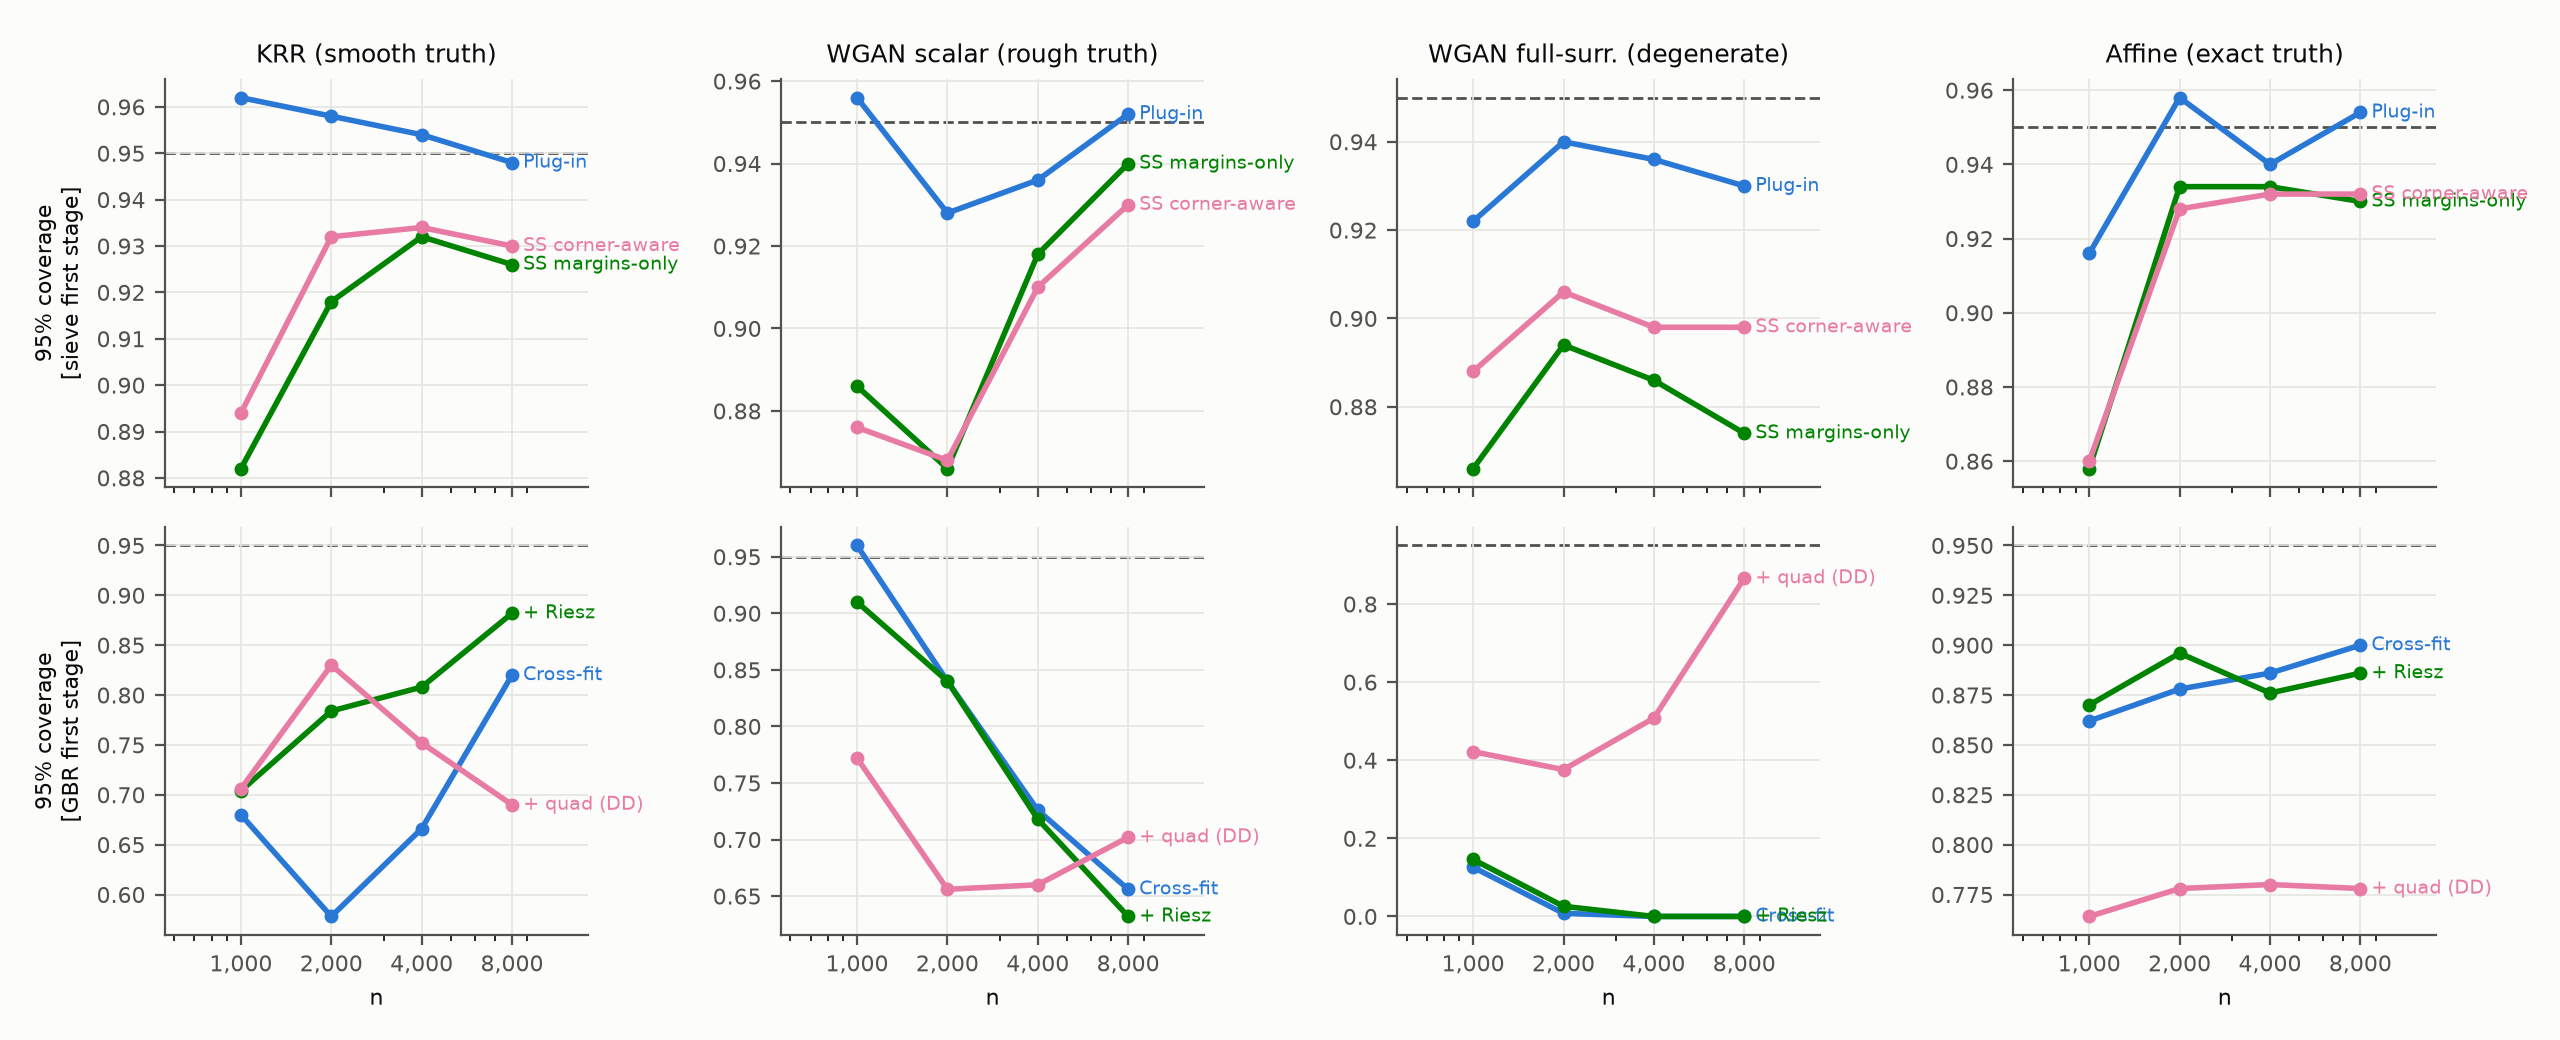
\includegraphics[width=\textwidth]{fig_debias_coverage.png}
\caption{Empirical 95\% coverage by sample size, DGP (columns), and
first-stage family (rows). Dashed line: nominal $0.95$.}
\label{fig:coverage}
\end{figure}

\begin{figure}[!htbp]
\centering
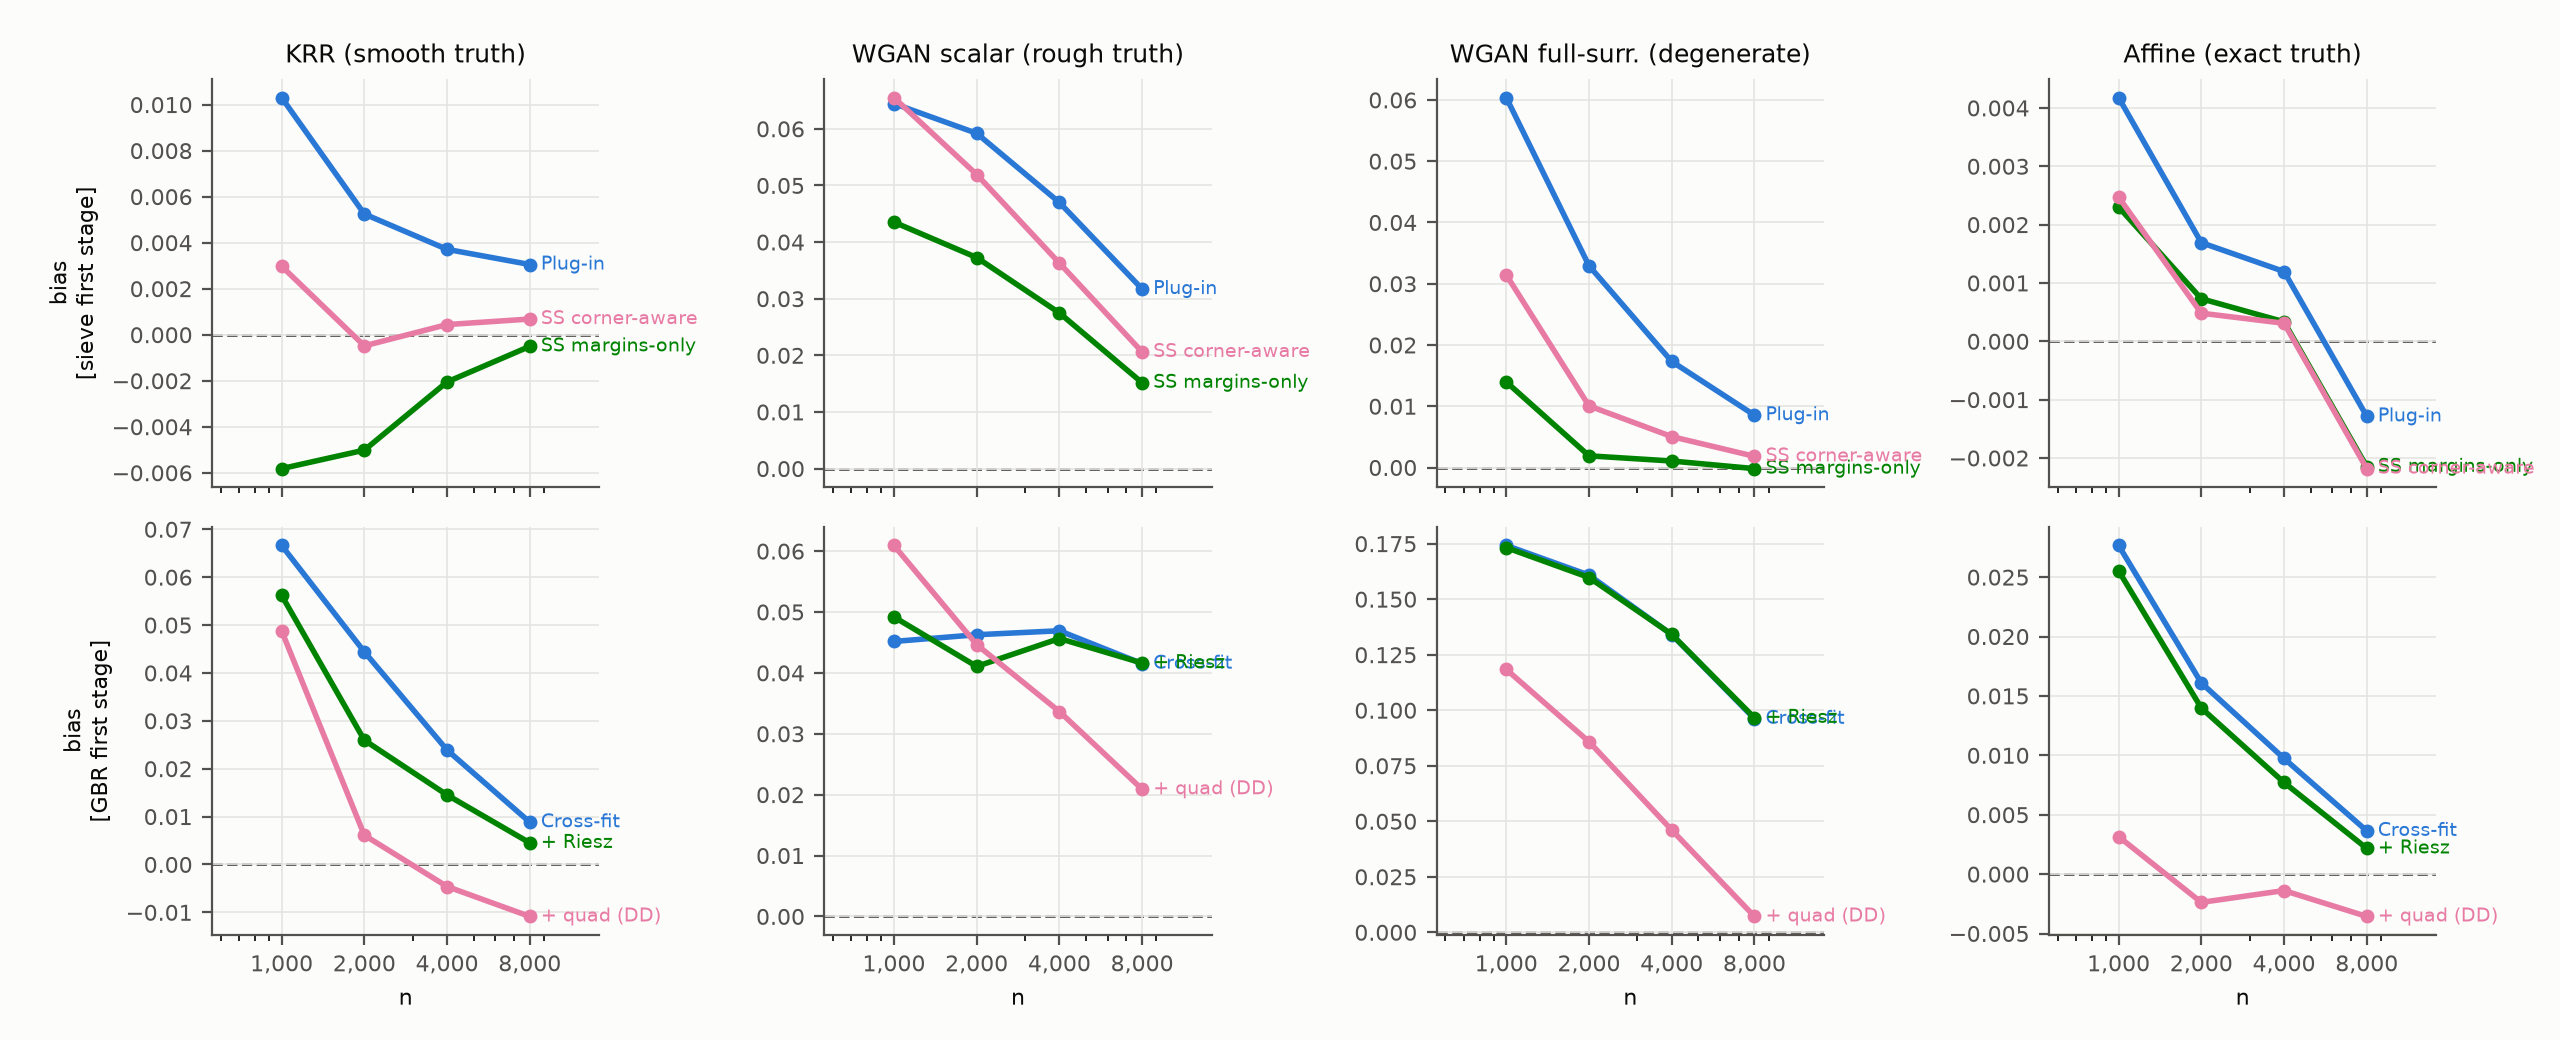
\includegraphics[width=\textwidth]{fig_debias_bias.png}
\caption{Monte Carlo bias by sample size, DGP, and estimator. Dashed
line: zero.}
\label{fig:bias}
\end{figure}

\begin{table}[!htbp]
\centering
\caption{Decomposition of the machine-learning undercoverage on the KRR
design ($n=4000$, $300$ replications). ``Plug-in bias'' is the uncorrected
cross-fit bias; ``bias'', ``SD'', ``SE/SD'', and ``coverage'' refer to the
Riesz-corrected estimator, studentized by \eqref{eq:two-band-var}. The
tensor-sieve plug-in is the reference. Varying folds, learner, and
representer basis one at a time isolates each mechanism of
Remark~\ref{rem:outofspan}.}
\label{tab:dml-diag}
\begin{tabular}{lccccc}
\toprule
Configuration & Bias & Plug-in bias & SD & SE/SD & Coverage \\
\midrule
%%DML_DIAG_TABLE_ROWS%%
tensor-sieve plug-in & +0.0034 & +0.0034 & 0.0178 & 1.03 & 0.943\\
gbr K=2 riesz=sieve & +0.0216 & +0.0317 & 0.0186 & 0.96 & 0.760\\
gbr K=5 riesz=sieve & +0.0106 & +0.0160 & 0.0191 & 0.94 & 0.903\\
gbr K=10 riesz=sieve & +0.0079 & +0.0127 & 0.0196 & 0.92 & 0.913\\
rf K=5 riesz=sieve & +0.0119 & +0.0453 & 0.0195 & 1.01 & 0.907\\
krr K=5 riesz=sieve & +0.0038 & +0.0039 & 0.0184 & 0.90 & 0.917\\
gbr K=5 riesz=rf & +0.0078 & +0.0160 & 0.0203 & 0.96 & 0.937\\
krr K=5 riesz=rf & +0.0047 & +0.0039 & 0.0181 & 0.98 & 0.937\\
gbr(high-cap) K=5 riesz=sieve & +0.0439 & +0.0461 & 0.0131 & 1.00 & 0.077\\
gbr K=5 no correction & +0.0160 & +0.0160 & 0.0189 & 0.94 & 0.857\\
\bottomrule
\end{tabular}
\end{table}

\begin{figure}[!htbp]
\centering
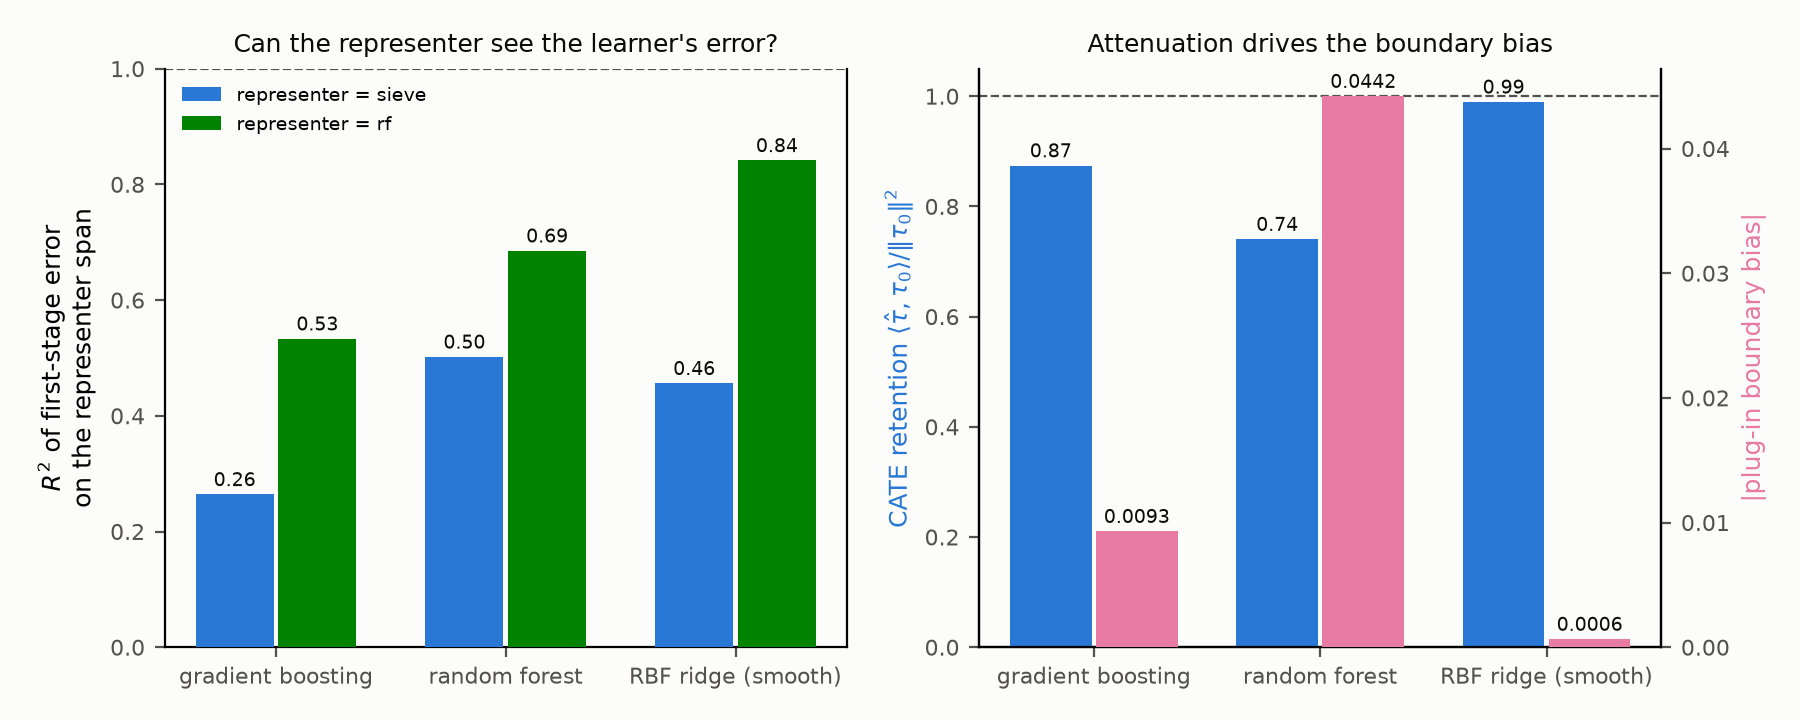
\includegraphics[width=\textwidth]{fig_dml_diagnosis.png}
\caption{Why boosting-based DML undercovers. \emph{Left}: the fraction
($R^{2}$) of the first-stage error that the sieve-Riesz representer can
span, measured against the oracle arm means; a boosted-tree error is largely
invisible to a smooth representer, a random-feature ridge's error is not.
\emph{Right}: tree learners attenuate the CATE (regression slope of fitted
on true $< 1$), which displaces the decision boundary and biases the
plug-in; the smooth learner barely attenuates and is nearly unbiased.}
\label{fig:dml-diag}
\end{figure}

\subsection{Corner anatomy: direct validation of the order claim}
\label{sec:anatomy}

Because the KRR oracle's contrast surfaces are known exactly, the corner set
and its geometry are computable: the zero curves of $\tau_{S}$ and $\tau_{Y}$
cross at ten points, with gradient norms
$\norm{\nabla\tau_{S}}\in[10.3,135.8]$, $\norm{\nabla\tau_{Y}}\in[13.9,56.4]$,
$\abs{\cos\omega}\leq0.90$ (transversality holds:
$\abs{\sin\omega}\geq0.45$), and within-unit residual correlation
$\rho_{SY}=0.524$. Table~\ref{tab:anatomy} traces the corner mechanism of
Section~\ref{sec:orders} across $300$ replications per sample size (sieve
first stage, fixed $K$).

\begin{table}[!htbp]
\centering
\caption{Corner anatomy on the KRR-calibrated oracle (300 reps, fixed
sieve dimension). ``Total'' is the implied plug-in corner bias
$\sum_{x^{*}}\E[\Delta_{g}\Delta_{h}]\,w/
(\norm{\nabla g_{0}}\norm{\nabla h_{0}}\abs{\sin\omega})$ in $\theta$ units;
``SS estimate'' is the mean corner cross correction
$\widehat{\text{corner}}$ of \eqref{eq:polarization}, which by split-sample
independence targets the \emph{stochastic} ($\rho_{SY}K/n$) part of the
diagonal; ``remainder'' is their difference, the bias-product
($K^{-2s/d}$) part. Sign convention: the anatomy script measures
$\E[\Delta\hat\tau_{S}\,\Delta\hat\tau_{Y}]$ (positive here, as
$\rho_{SY}>0$); the table reports the corner term in $\theta$ units, where
the harm-share convention $h_{0}=-\tau_{Y}$ flips its sign. $\overline{\text{corr}}$ averages
$\mathrm{Corr}(\Delta_{g}(x^{*}),\Delta_{h}(x^{*}))$ over the ten corners.}
\label{tab:anatomy}
\begin{tabular}{lccccc}
\toprule
$n$ & Total corner bias & SS estimate & Remainder &
$\overline{\text{corr}}(\Delta_{g},\Delta_{h})$ & $\rho_{SY}$\\
\midrule
2000 & $-0.0080$ & $-0.0044$ & $-0.0036$ & $0.50$ & $0.524$\\
4000 & $-0.0048$ & $-0.0022$ & $-0.0025$ & $0.46$ & $0.524$\\
8000 & $-0.0038$ & $-0.0012$ & $-0.0026$ & $0.45$ & $0.524$\\
\bottomrule
\end{tabular}
\end{table}

Three predictions of Section~\ref{sec:orders} are confirmed jointly.
\emph{(i)} The pointwise correlation of the two surface errors at the corner
equals the within-unit residual correlation ($0.45$--$0.50$ against
$\rho_{SY}=0.524$), which is the mechanism behind the
$\rho_{SY}K_{n}/n$ term in \eqref{eq:corner-order}. \emph{(ii)} The
stochastic part of the corner diagonal halves as $n$ doubles at fixed $K$
($-0.0044\to-0.0022\to-0.0012$) --- the $K/n$ scaling --- and is tracked by
the SS corner correction, which by construction cancels bias parts across the
two independent halves. \emph{(iii)} The remainder is roughly constant in $n$ at
fixed $K$ ($-0.0036$ at $n=2000$, then $\approx-0.0025$), as befits the
$K^{-2s/d}$ bias product, which
is controlled by undersmoothing $K$ rather than by debiasing. The total
corner bias ($0.4$--$0.8$ percentage points of a $\theta_{0}=0.161$ target)
is material relative to the plug-in standard error, and its sign
($\rho_{SY}>0$ pushes the plug-in \emph{down} here after the
$h=-\tau_{Y}$ sign flip) matches the Monte Carlo finding that the
corner-aware and margins-only SS estimates differ by
$+0.004$ to $+0.005$ at $n=2000$.

\subsection{Results}\label{sec:results}

Table~\ref{tab:mc-main} and Figures~\ref{fig:coverage}--\ref{fig:bias}
report all cells. The theoretical predictions play out as follows.

\emph{(1) Smooth truth (KRR): the plug-in is already good; corner-aware SS
removes what bias there is.} The plug-in covers at $0.948$--$0.962$ at all
$n$ with a small decaying bias ($+0.010\to+0.003$) and a well-calibrated
standard error (SE/SD $0.94$--$1.11$, tightening toward one with $n$). SS
debiasing removes the bias
essentially completely ($+0.003\to+0.0007$; a $3.5$-fold bias reduction at
$n=1000$ and a tenfold reduction at $n=2000$) at negligible variance cost
by $n\geq4000$. Decisively for the
theory, the \emph{margins-only} correction overshoots to negative bias
($-0.006$ to $-0.0005$) at every $n$: it removes the (positive) margin
diagonals but not the (negative, $\rho_{SY}$-driven) corner term. The gap
between the corner-aware and margins-only estimates equals the estimated
corner correction ($\hat\Th_{SS}=\hat\Th_{SS}^{\text{mar}}
-\widehat{\text{corner}}$) and matches the anatomy of
Table~\ref{tab:anatomy} to the fourth decimal ($+0.0045$ at $n=2000$
against minus the anatomy's SS corner estimate of $-0.0044$).
The raw corner cross form $q_{\text{full}}-q_{g}-q_{h}$ (eight times the
corner correction) halves as $n$ doubles
($-0.070\to-0.036\to-0.020\to-0.0095$), the $K_{n}/n$ scaling of
\eqref{eq:corner-order}.

\emph{(2) Rough truth (scalar WGAN, $s\approx1$): debiasing accelerates the
bias decay and preserves honest coverage.} The plug-in bias is large and
decays at only $\approx n^{-0.34}$ ($+0.064\to+0.032$), and its near-nominal
coverage rests on a conservative SE (SE/SD $1.1$--$1.3$). SS debiasing
accelerates the decay to $\approx n^{-0.55}$ ($+0.066\to+0.021$) with an
honest SE (SE/SD $0.83$--$0.98$, $\approx0.95$ for $n\geq4000$) and
coverage converging to $0.93$--$0.94$ at $n=8000$. On this rough truth the margins-only variant is slightly
better centered than the corner-aware one --- with $s\approx1$ the corner
correction is itself noisily estimated --- a useful caution: corner-awareness
is a bias-\emph{decomposition} necessity (KRR shows the corner term is real
and quantitatively predictable), but its sampled version adds noise when
the surfaces are rough.

\emph{(3) Machine-learning first stages: the projected Riesz correction
works where the learner is adequate; the quadratic correction is not a free
lunch.} On the smooth truth the GBR bias falls monotonically along the
ladder cross-fit $\to$ $+$Riesz $\to$ $+$quadratic at every $n$ (at
$n=4000$: $+0.024\to+0.015\to-0.005$), confirming that the two corrections
target distinct error terms. But the composition has two finite-sample
costs: the SS-on-GBR quadratic correction inflates the dispersion (by a
factor of two at $n=1000$, $1.4$ thereafter), and the first-order SE does
not account for it (SE/SD $\approx0.6$), so DD
intervals undercover ($0.69$--$0.83$); and at $n=8000$ on KRR the
quadratic correction overshoots ($-0.011$) --- boosting error is not
``linear plus small quadratic,'' so the third-order smallness condition of
Theorem~\ref{thm:dd} fails for these learners at these sample sizes. On the
rough truth GBR is simply bias-limited ($+0.045$ nearly flat in $n$;
coverage falls to $0.64$): no first-order correction can rescue a nuisance
that misses the kinks. The degenerate arm is the extreme case: GBR
manufactures a spurious harm share of $+0.17$ (coverage $0$), and there the
quadratic correction \emph{does} rescue it asymptotically
($+0.007$, coverage $0.87$ at $n=8000$).

\emph{(4) The two-band SE is well calibrated for the sieve family.} The
variance estimator \eqref{eq:two-band-var} includes the empirical-measure
term $\theta(1-\theta)/n$ --- the sampling error of the average given the
surfaces, the exact analogue of the $\mathrm{Var}([h_{0}]_{+})$ term the
single-threshold unknown-density welfare theorem adds --- which is $6$--$12\%$
of the SE at these sample sizes and, if omitted, produces a spurious
SE/SD of $0.87$--$0.95$. With it included, SE/SD is $0.90$--$1.11$ for
plug-in and SS on the KRR and affine designs, and the studentized intervals
reach $0.93$--$0.95$ by $n=8000$; on the degenerate arm ($\theta_{0}=0$,
empty margins) the sieve family degrades gracefully.

\emph{(5) Machine-learning first stages: why the sieve-DML interval
undercovers, and when it does not.} The cross-fitted GBR estimators cover
only $0.58$--$0.88$ on the smooth design, in sharp contrast to the sieve
plug-in on the \emph{same samples} --- so the shortfall is a property of the
first stage, not the DGP or the variance formula. The diagnosis is
Remark~\ref{rem:outofspan}. Measured against the oracle arm means, the
$R^{2}$ of the boosted first-stage error on the tensor B-spline representer
span is only $0.26$; the projected correction therefore removes just
$31\%$ of the plug-in's boundary bias, and by the variance-addition identity
of Remark~\ref{rem:outofspan} the leftover is independent of the score, so
the SE (which estimates only $\sigma_{n}^{2}/n$) understates the dispersion.
Three levers move coverage exactly as the theory predicts:
\emph{(i) folds} --- $K=2\to5\to10$ lifts GBR coverage $0.76\to0.90\to0.91$
by shrinking the own-observation bias trained on $(K-1)/K$ of the sample;
\emph{(ii) representer basis} --- matching a $400$-feature random-feature
representer to the boosted learner raises the projected $R^{2}$ from $0.26$
to $0.53$ and coverage from $0.90$ to $0.94$; \emph{(iii) learner
smoothness} --- a random-feature (RBF) ridge, whose error the representer
\emph{can} span ($R^{2}=0.84$), attenuates the CATE by only $1\%$ (against
boosting's $13\%$) and has a plug-in bias of $+0.0006$ (against $+0.016$),
so there is almost nothing left to correct and, with a matched representer,
it too reaches $0.94$. Higher-capacity boosting is
counterproductive --- it sharpens the axis-aligned staircase, driving
coverage toward zero. The pattern reproduces the parent draft's own
single-threshold Table~7 (boosting: unbiased but SE/SD $=0.78$--$0.88$,
coverage stuck at $0.90$; smooth learner: SE/SD up to $0.99$). The residual
$0.01$--$0.02$ shortfall of even the best machine-learning cell below the
sieve plug-in's coverage is the out-of-span component the standard error
cannot see, exactly as Remark~\ref{rem:outofspan} predicts.

\emph{Practical guidance.} For sieve first stages, use the corner-aware SS
estimator \eqref{eq:jackknife} with the two-band SE: it is tuning-free,
removes the second-order bias including the corner, and its interval is
honest. For a machine-learning first stage --- needed when $d$ is too large
for a tensor sieve --- prefer a \emph{smooth} learner and \emph{match the
representer basis to the learner's own feature map}, so the projected
correction is near-exact; avoid tree ensembles, whose piecewise-constant
error is largest precisely on the margins the representer must span, and
never use $2$-fold cross-fitting for the point estimate. When a tree first
stage is unavoidable, pair it with a full-refit bootstrap rather than the
analytic SE. The comparison of the corner-aware and margins-only corrections
is a useful specification diagnostic in its own right: their gap estimates
the corner term, whose magnitude flags whether the two-threshold structure
is quantitatively binding.

\appendix

\section{Derivation of the Second Derivative (Theorem~\ref{thm:D2})}
\label{app:D2}

Write $T_{g}(t):=\int_{\{g_{t}=0\}\cap\{h_{t}\geq0\}}
\varpi_{t}\dd\Haus^{d-1}$ with weight
$\varpi_{t}:=u\,w/\norm{\nabla g_{t}}$ (we reserve $\omega(x)$ for the
transversality angle throughout), the first term of \eqref{eq:D1}
along $\gamma_{t}$; the second term is symmetric. Let
${\bf X}(\cdot,t)$ be the normal diffeomorphism carrying
$\mathcal M:=\{g_{0}=0\}$ to $\{g_{t}=0\}$ with velocity
$\dot{\bf X}=-(u/\norm{\nabla g_{0}})\,n_{g}$, and pull the integral back
to $\mathcal M$:
\[
T_{g}(t)=\int_{\mathcal M}
\1\{h_{t}({\bf X}(x,t))\geq0\}\;
\varpi_{t}({\bf X}(x,t))\,J_{\bf X}(x,t)\dd\Haus^{d-1}(x).
\]
Differentiating at $t=0$ yields four contributions.
\emph{(1) Integrand:} $\partial_{t}\varpi_{t}
=-u\,w\,(n_{g}\!\cdot\!\nabla u)/\norm{\nabla g_{0}}^{2}$.
\emph{(2) Transport of $\varpi$ and area:} by the surface-transport formula
(Delfour and Zol\'esio, 2001, Ch.~9),
$\partial_{t}\{\varpi({\bf X})J_{\bf X}\}
=-\big[(u/\norm{\nabla g_{0}})\,n_{g}\!\cdot\!\nabla\varpi
+\varpi\,(u/\norm{\nabla g_{0}})H_{g}\big]$, the moving-level-set terms of
Chen and Gao (2026, Lem.~PathD--Level) with weight $\varpi$.
\emph{(3) Direct motion of the cut:} the indicator
$\1\{h_{t}\geq0\}$ evaluated on the (fixed, $t=0$) manifold defines the
region $\{h_{0}+tv\geq0\}\cap\mathcal M$; by the within-manifold Leibniz
rule its derivative is an integral over the relative boundary
$\Corner$ with normal velocity $v/\norm{\nabla_{\!\mathcal M}h_{0}}$, where
$\norm{\nabla_{\!\mathcal M}h_{0}}=\norm{P_{T}\nabla h_{0}}
=\norm{\nabla h_{0}}\abs{\sin\omega}$, giving
$+\int_{\Corner}\varpi_{0}\,v/(\norm{\nabla h_{0}}\abs{\sin\omega})
\dd\Haus^{d-2}$ --- the cross term.
\emph{(4) Induced motion of the cut:} the composition
$h_{0}({\bf X}(x,t))=h_{0}(x)-t\,(u/\norm{\nabla g_{0}})\,
n_{g}\!\cdot\!\nabla h_{0}+o(t)
=h_{0}(x)-t\,u\,\norm{\nabla h_{0}}\cos\omega/\norm{\nabla g_{0}}+o(t)$
perturbs the cut function by an effective
$v_{\text{eff}}=-u\norm{\nabla h_{0}}\cos\omega/\norm{\nabla g_{0}}$;
the same within-manifold Leibniz rule then contributes
$-\int_{\Corner}\varpi_{0}\,u\cos\omega/
(\norm{\nabla g_{0}}\abs{\sin\omega})\dd\Haus^{d-2}$ --- the diagonal
corner term of \eqref{eq:Qg}. Collecting (1)--(4), and adding the symmetric
derivative of the $\Mh$-term (which contributes the mirror-image margin
form, the second copy of the cross term, and the $v^{2}$ diagonal corner
term), gives \eqref{eq:D2}--\eqref{eq:Qg}. Transversality bounds every
corner integrand; twice-differentiability of $g_{0},h_{0}$ and
Assumption~\ref{ass:model}(d) bound the curvature and gradient terms.
$\hfill\square$

\section{Remarks on the Proofs of
Theorems~\ref{thm:ss}--\ref{thm:dd}}\label{app:proofs}

The margin components of all remainder bounds are direct adaptations of the
single-threshold arguments --- Chen and Gao (2026, Thms.~5, 8 and the SS/LOO
constructions) for the quadratic terms, and the extended single-threshold
draft (sieve-DML theorem and its Assumption~5) for the cross-fitted
first-order correction --- applied margin by margin with the truncation
indicators carried as bounded weights. The new ingredients are (i) the
corner terms of Theorem~\ref{thm:D2}, whose diagonals are removed by the SS
correction exactly as the margin diagonals are (the split-sample
independence argument is dimension-free), and whose off-diagonal cross-half
parts are degenerate second-order U-statistics over a
$(d-2)$-dimensional set, hence of strictly smaller order than the margin
off-diagonals; and (ii) the joint CLT for the two-band linear term, which
follows from the Cram\'er--Wold device and the Lindeberg condition applied
to the summed per-unit influence
$v^{*}_{S}(X_{i},W_{i})\epsilon_{S,i}+v^{*}_{Y}(X_{i},W_{i})\epsilon_{Y,i}$
--- the within-unit correlation $\rho_{SY}$ is absorbed into
$\sigma_{n}^{2}$ by construction \eqref{eq:two-band-var}. Complete proofs
are being written for the full paper draft; every statement above is
formulated so that the cited single-threshold lemmas apply to the margin
parts verbatim, and the corner parts require only the transversality bound
and the dimension count $\dim\Corner=d-2$.

\bigskip
\noindent\textbf{References} (to be merged into \texttt{JMP.bib}):
Athey, Chetty, Imbens, Kang (2024) surrogate index; Banerjee et al.\ (2015)
graduation RCT; Chen and Ritzwoller (2023) semiparametric long-term
estimation and WGAN calibration; Athey, Imbens, Metzger, Munro (2021)
ds-WGAN; Chen, Chen, Gao (2025) single-threshold welfare/value inference and
its extended draft (quadratic debiasing, sieve DML); Chen and Gao (2026)
thin-set minimax theory; Delfour and Zol\'esio (2001) shape calculus; Evans
and Gariepy (2015) coarea/band limits.

\end{document}
